\documentclass[../Main.tex]{subfiles}
\begin{document}
In the fourth chapter of this dissertation, we delve into the complexities and technical aspects of our innovative social authentication system. It is a comprehensive guide for comprehending the architecture, design, and implementation of the system. This chapter provides a detailed analysis of a number of crucial components, casting light on the obstacles encountered during development and the solutions employed to overcome them.
\section{Requirement analysis}
\subsection{General usecases diagram}
\begin{figure}[H]
 \centering
 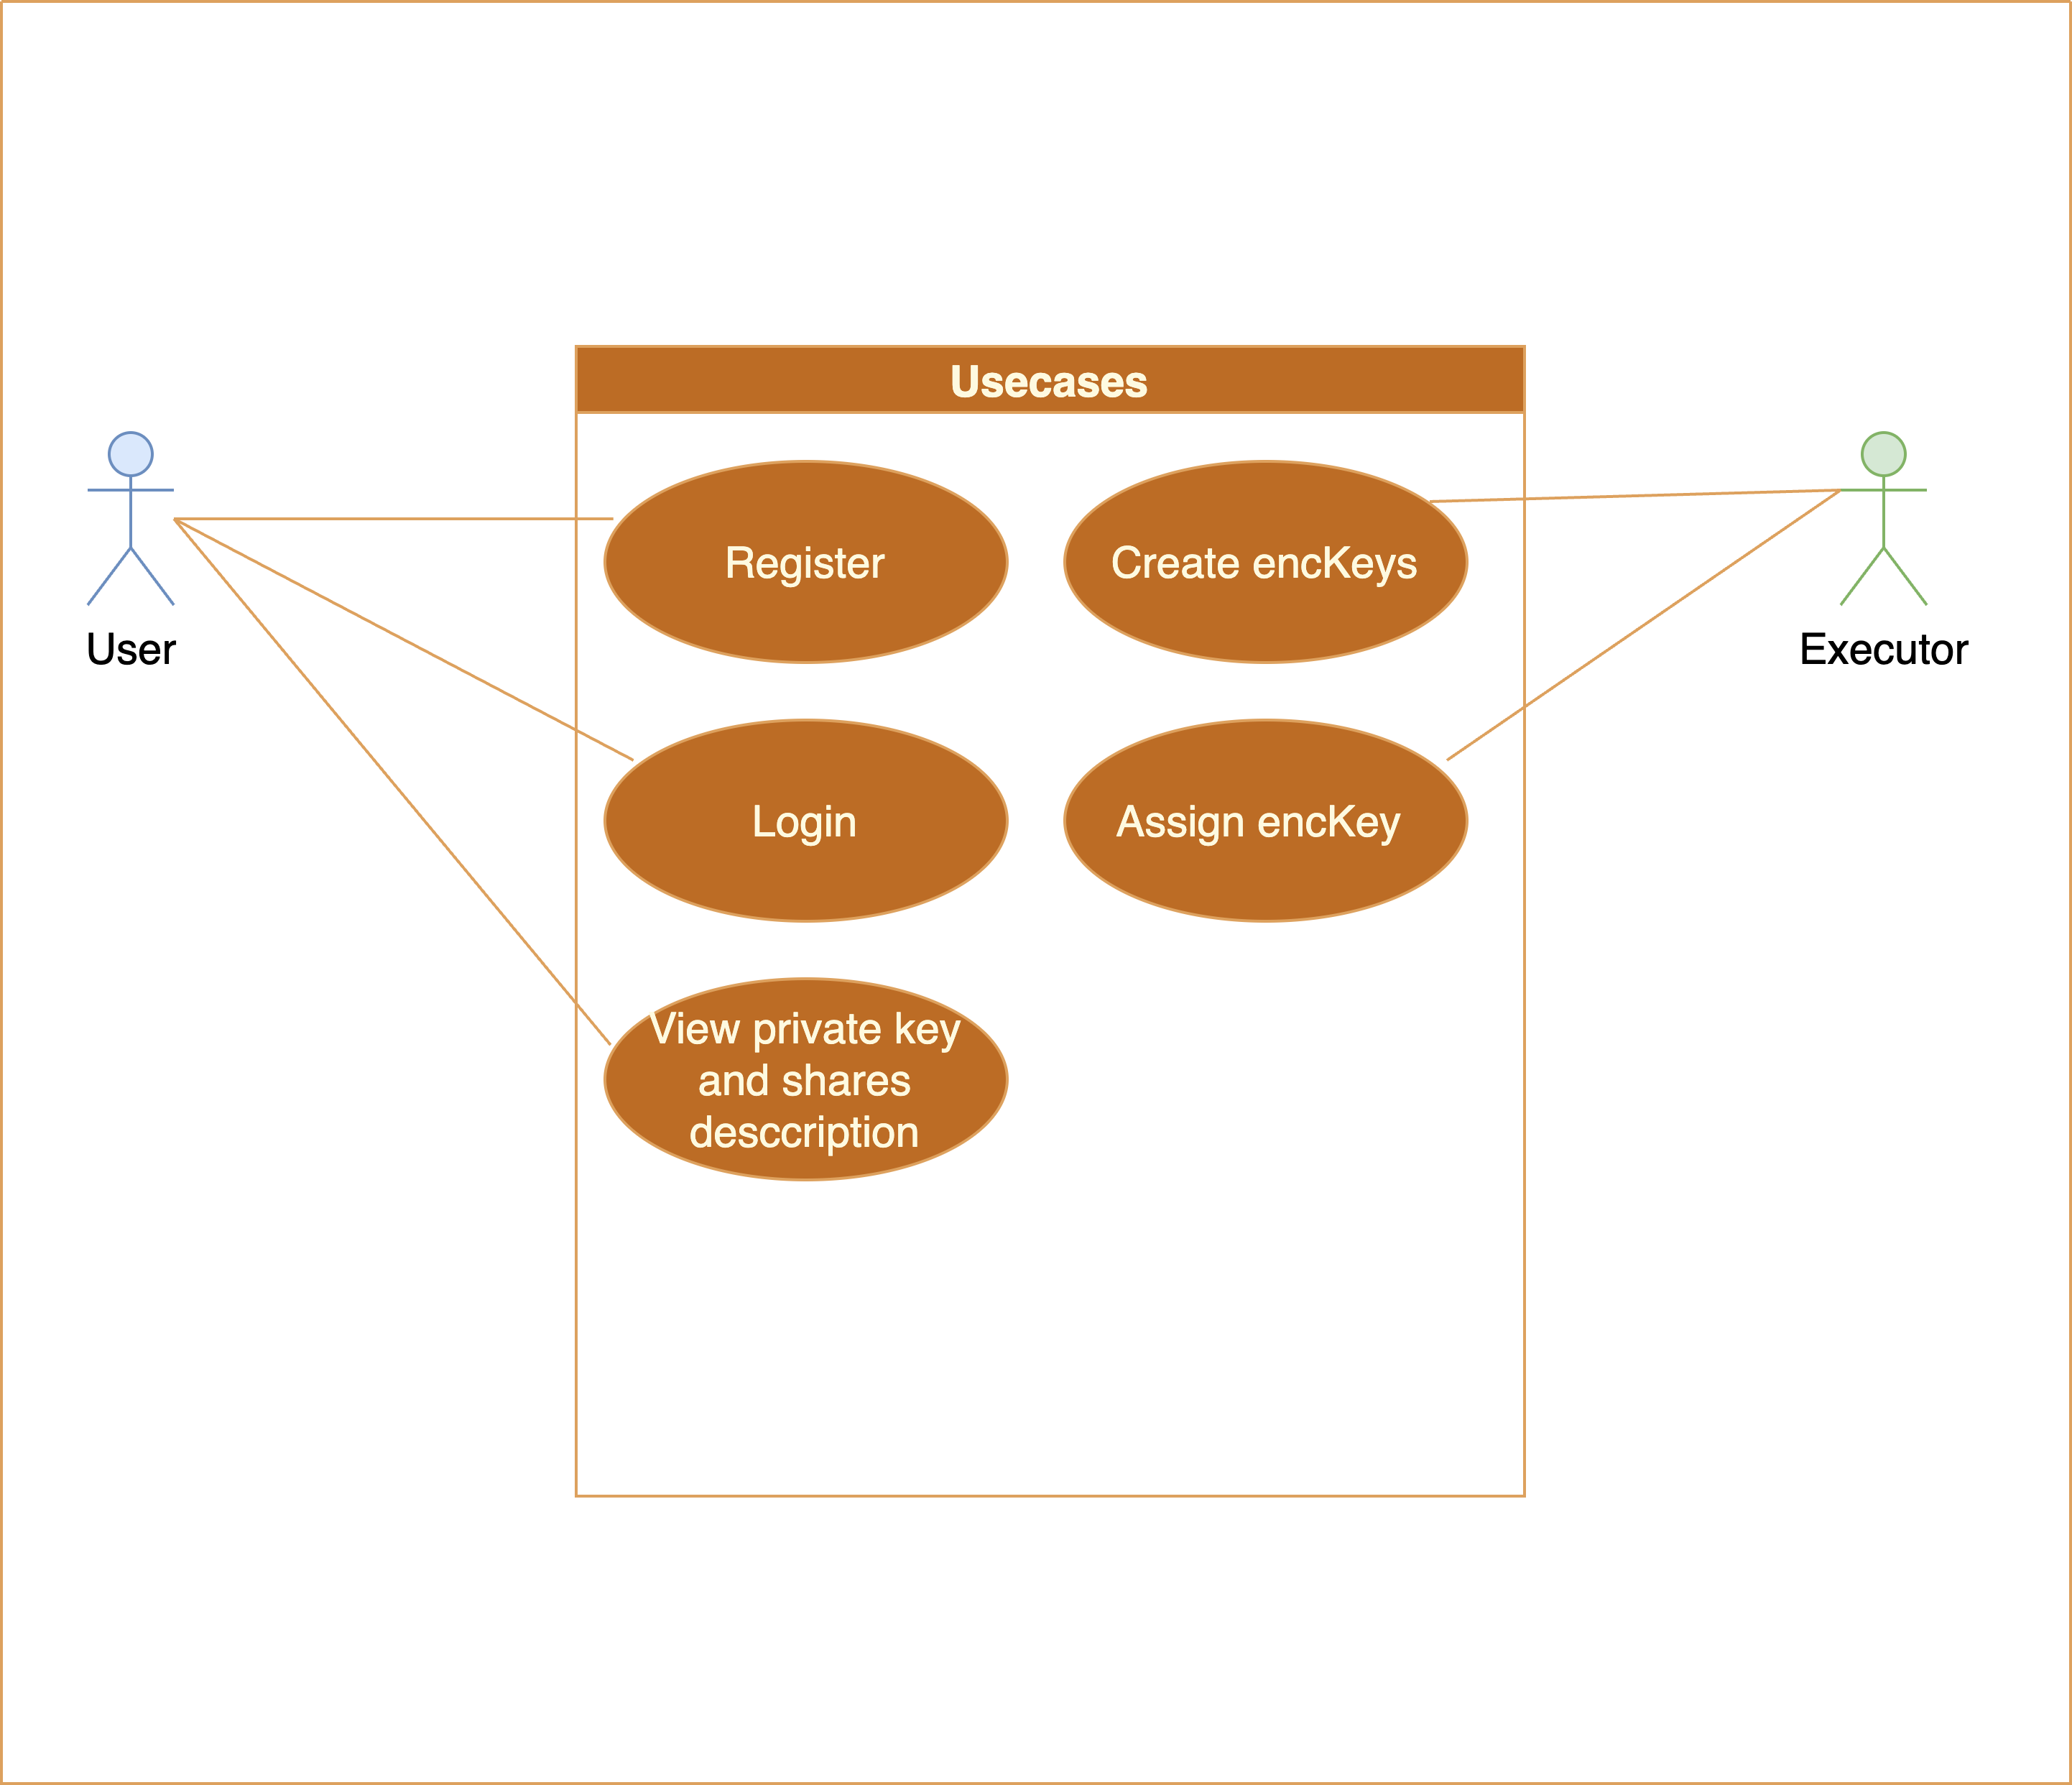
\includegraphics[scale=0.14]{Figure/general-usecases.png}
 \caption{General usecases diagram}
    \label{fig:general-usecases}
\end{figure}
The figure \ref{fig:general-usecases} depicts the general usecases of Social login system. There are two actors included in the system.
The first one is User who will use the main function social login. The table below describes more detail about functionalities of usecase:\\
\begin{table}[H]
  \centering
  \begin{tabular}{|c|p{3cm}|p{9cm}|}
  \hline
  \textbf{No} & \textbf{Use Case} & \textbf{Description} \\
  \hline
  1 & Regiser & User using their social account such as: Google, facebook, ... for signing up the web3 spaces\\
  \hline
  2 & Login & User using their social account such as: Google, facebook, ... for  signing in the web3 spaces\\
  \hline
  3 & View the private key and shares description & User fully controls and manages their private key and their shares.\\
  \hline
  \end{tabular}
  \caption{User's usecase description}
  \label{user-usecase}
\end{table}

The second participant is the Executor. They are special users with a crucial function who run the system's create encKey and assign encKey processes in the background.

\begin{table}[H]
  \centering
  \begin{tabular}{|c|p{3cm}|p{9cm}|}
  \hline
  \textbf{No} & \textbf{Use Case} & \textbf{Description} \\
  \hline
  1 & Create encKey & Executor run the phases of Pedersen Protocol for pre-creating the encKey for user to encrypt their share.\\

  \hline
  2 & Provide signature & Executors communicate with one another via signatures; if the number of valid signatures exceeds the threshold, anyone can delegate a key to a specific user via a multi-signature mechanism.\\
  \hline
  \end{tabular}
  \caption{Executor's usecase description}
  \label{executor-usecase}
\end{table}
\subsection{Usecase specifications and activity diagrams}
For a better understanding of the use cases, I'd like to include the corresponding activity diagrams beneath each specification.
% User usecase

\begin{table}[H]
  \centering
  \begin{tabular}{|
  >{\columncolor[HTML]{32CB00}}l |lll|}
  \hline
  \textbf{Usecase code}       & \multicolumn{1}{l|}{UC001} & \multicolumn{1}{l|}{\textbf{Usecase name}} & Social login \\ \hline
  \textbf{Actor}              & \multicolumn{3}{l|}{User}                                                              \\ \hline
  \textbf{Pre-condition}       & \multicolumn{3}{l|}{At least have 1 social account}                                    \\ \hline
  \textbf{Main flow of event} & \multicolumn{3}{l|}{
            \begin{tabular}{|
              >{\columncolor[HTML]{FFFFFF}}p{2cm}|p{3cm}|p{6cm}|}
                  \hline
                  \cellcolor[HTML]{F56B00}\textbf{No} & \cellcolor[HTML]{F56B00}\textbf{Actor} & \cellcolor[HTML]{F56B00}\textbf{Action} \\ \hline
                  \textbf{1}                          & User                                   &  Select social login type    \\ \hline
                  \textbf{2}                          & System                                       &  Redirect to authorize\\ \hline
                  \textbf{3}                          & Auth0                                       &  Redirect to login and authorization form  \\ \hline
                  \textbf{4}                          & User                                       & Authenticate and consent                                         \\ \hline
                  \textbf{5}                          & Auth0                                       & Redirect with single use authorization code\\ \hline
                  \textbf{6}                          & System                                  & Send code clientId and credentials to get oauth token\\ \hline
                  \textbf{7}                          & Auth0                                   & Verify code, cliendId, credentials \\ \hline
                  \textbf{8}                          & Auth0                                   & Send idToken, access token and refresh token\\ \hline
                  \textbf{9}                          & System                                  & Authenticate the idToken or access token\\ \hline
                  \textbf{10}                          & System                                  & Assign encKey for user\\ \hline
                  \textbf{11}                          & System                                  & Send shares \\ \hline
                  \textbf{12}                          & System                                  & Contruct the encKey \\ \hline
                  \textbf{13}                          & System                                  & Construct the private Key \\ \hline
            \end{tabular}
  } \\ \hline
  \textbf{Alternative flow of event} & \multicolumn{3}{l|}{
            \begin{tabular}{|
              >{\columncolor[HTML]{FFFFFF}}p{2cm}|p{3cm}|p{6cm}|}
                  \hline
                  \cellcolor[HTML]{F56B00}\textbf{No} & \cellcolor[HTML]{F56B00}\textbf{Actor} & \cellcolor[HTML]{F56B00}\textbf{Action} \\ \hline
                  \textbf{5b}                          & Auth0    &  Return error if the authenticate and consent fail or rejected\\ \hline
                  \textbf{8b}                          & Auth0    &  Response with error because fail in verification\\ \hline
            \end{tabular}
  }
  \end{tabular}
    \caption{Sign up specification}
    \label{sign-up-specification}
  \end{table}
\begin{figure}[H]
 \centering
 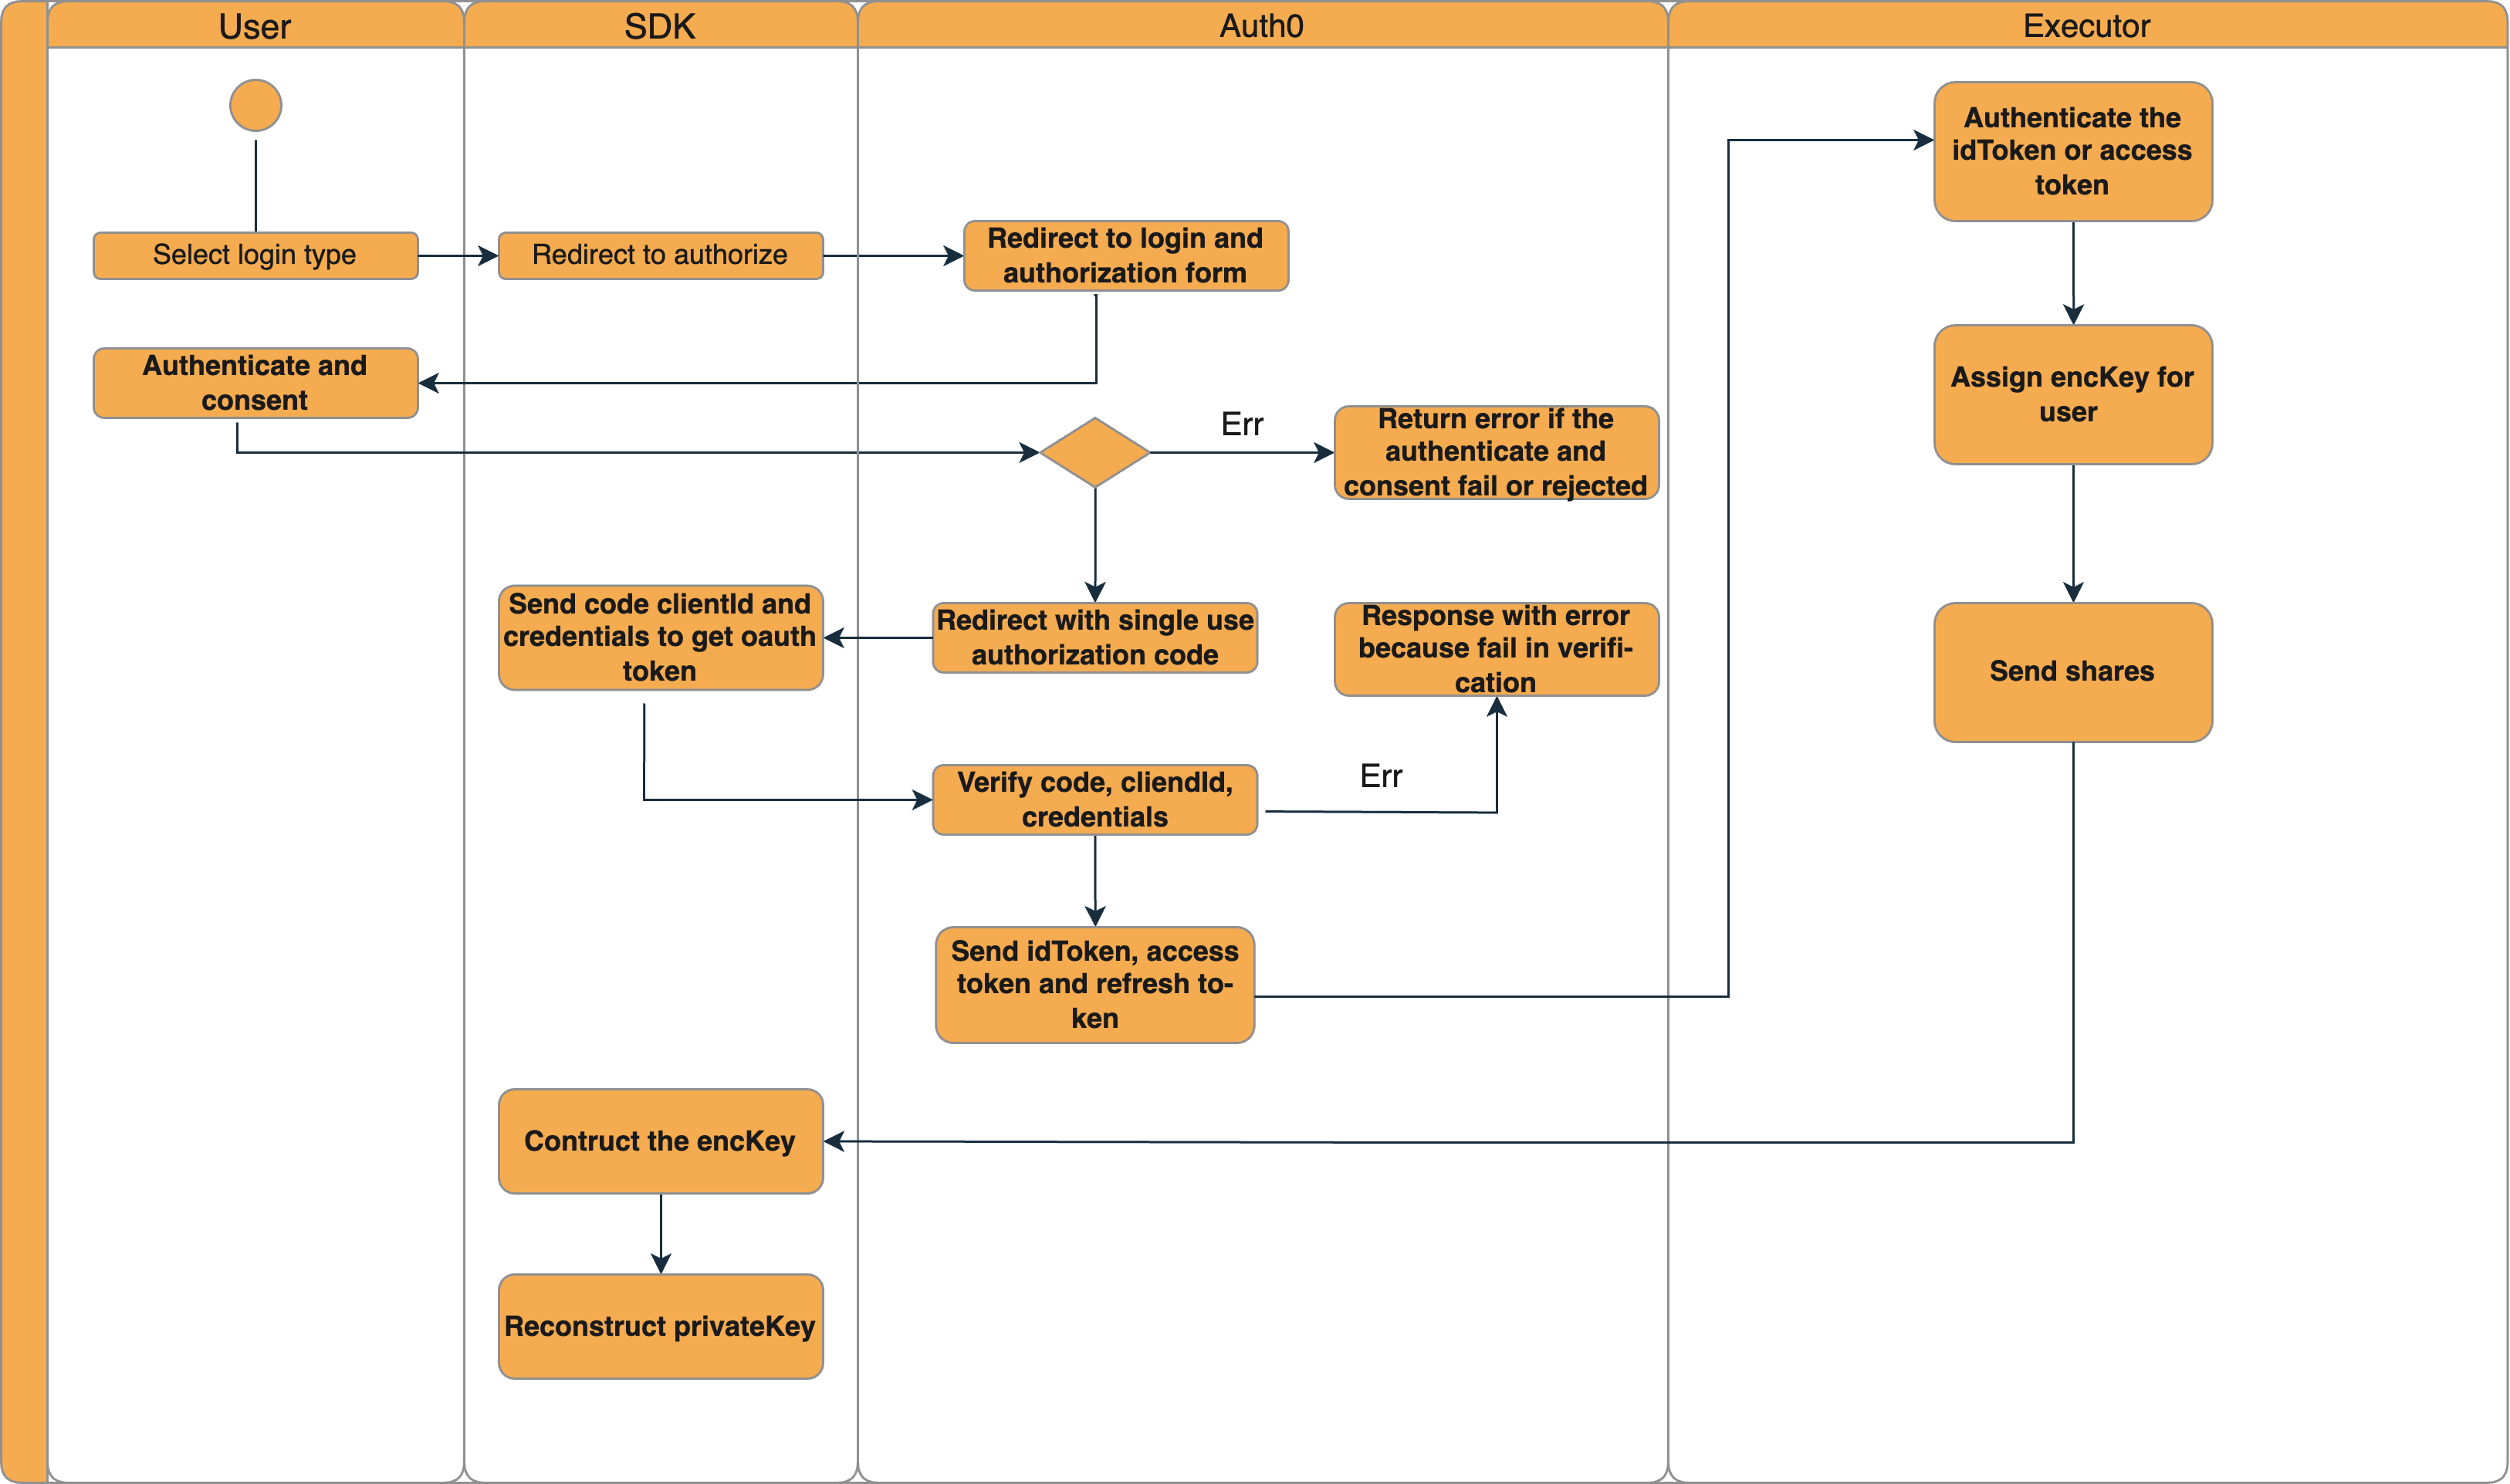
\includegraphics[scale=0.14]{Figure/sign-up-activity.png}
 \caption{Signing up activity}
    \label{fig:sign-up-activity}
\end{figure}
  Figure \ref{fig:sign-up-activity} is an activity diagram that illustrates the process, how users interact with the system, and the connections between the components. The SDK acts as a bridge between users and the remainder of the system, while Executors and Auth0 validate users' identities. In addition, executors assign and provide the requirements for user encKey and private key construction.

\begin{table}[H]
  \centering
  \begin{tabular}{|
  >{\columncolor[HTML]{32CB00}}l |lll|}
  \hline
  \textbf{Usecase code}       & \multicolumn{1}{l|}{UC001} & \multicolumn{1}{l|}{\textbf{Usecase name}} & Social login \\ \hline
  \textbf{Actor}              & \multicolumn{3}{l|}{User}                                                              \\ \hline
  \textbf{Pre-condition}       & \multicolumn{3}{l|}{At least have 1 social account}                                    \\ \hline
  \textbf{Main flow of event} & \multicolumn{3}{l|}{
            \begin{tabular}{|
              >{\columncolor[HTML]{FFFFFF}}p{2cm}|p{3cm}|p{6cm}|}
                  \hline
                  \cellcolor[HTML]{F56B00}\textbf{No} & \cellcolor[HTML]{F56B00}\textbf{Actor} & \cellcolor[HTML]{F56B00}\textbf{Action} \\ \hline
                  \textbf{1}                          & User                                   &  Select social login type    \\ \hline
                  \textbf{2}                          & System                                       &  Redirect to authorize\\ \hline
                  \textbf{3}                          & Auth0                                       &  Redirect to login and authorization form  \\ \hline
                  \textbf{4}                          & User                                       & Authenticate and consent                                         \\ \hline
                  \textbf{5}                          & Auth0                                       & Redirect with single use authorization code\\ \hline
                  \textbf{6}                          & System                                  & Send code clientId and credentials to get oauth token\\ \hline
                  \textbf{7}                          & Auth0                                   & Verify code, cliendId, credentials \\ \hline
                  \textbf{8}                          & Auth0                                   & Send idToken, access token and refresh token\\ \hline
                  \textbf{9}                          & System                                  & Authenticate the idToken or access token\\ \hline
                  \textbf{10}                          & System                                  & Send shares \\ \hline
                  \textbf{11}                          & System                                  & Contruct the encKey \\ \hline
                  \textbf{12}                          & System                                  & Construct the private Key \\ \hline
            \end{tabular}
  } \\ \hline
  \textbf{Alternative flow of event} & \multicolumn{3}{l|}{
            \begin{tabular}{|
              >{\columncolor[HTML]{FFFFFF}}p{2cm}|p{3cm}|p{6cm}|}
                  \hline
                  \cellcolor[HTML]{F56B00}\textbf{No} & \cellcolor[HTML]{F56B00}\textbf{Actor} & \cellcolor[HTML]{F56B00}\textbf{Action} \\ \hline
                  \textbf{5b}                          & Auth0    &  Return error if the authenticate and consent fail or rejected\\ \hline
                  \textbf{8b}                          & Auth0    &  Response with error because fail in verification\\ \hline
            \end{tabular}
  }
  \end{tabular}
    \caption{Sign in specification}
    \label{sign-in-specification}
  \end{table}
\begin{figure}[H]
 \centering
 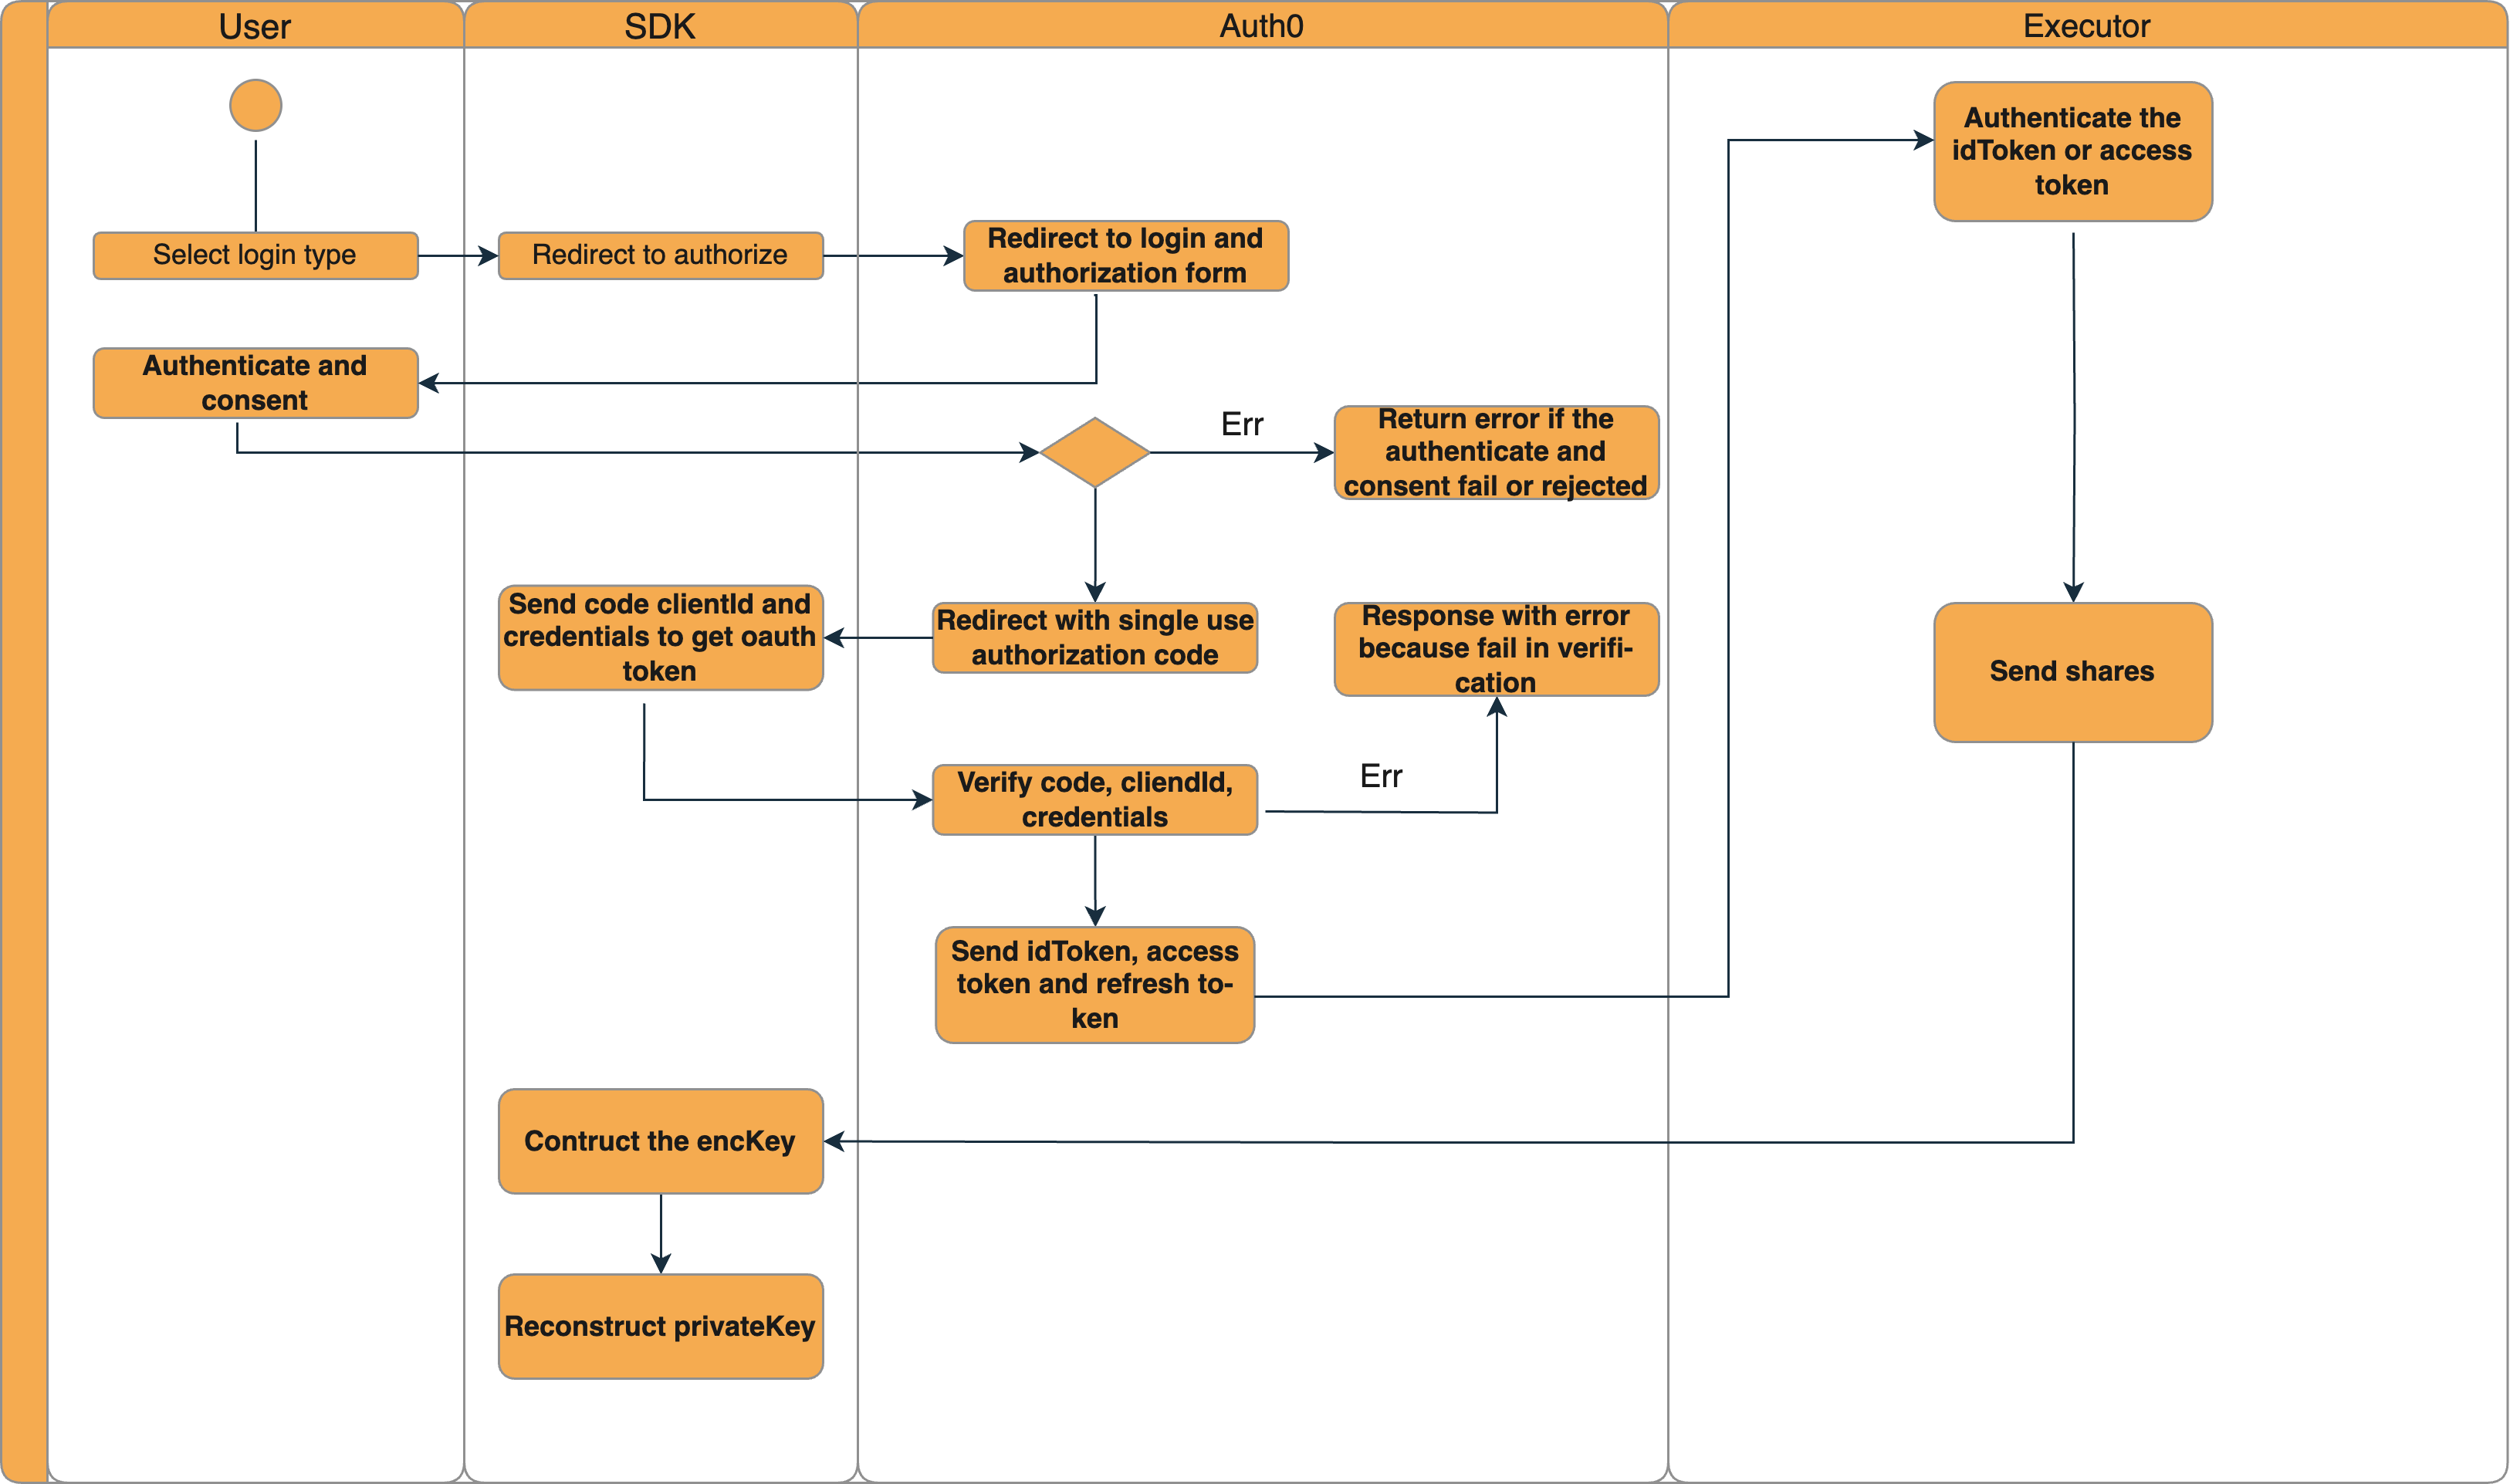
\includegraphics[scale=0.14]{Figure/sign-in-activity.png}
 \caption{Signing in activity}
    \label{fig:sign-in-activity}
\end{figure}
  Similar to figure \ref{fig:sign-up-activity}, figure \ref{fig:sign-in-activity} describes in detail how users login into the system and how the system's components interact. 

\begin{table}[H]
  \centering
  \begin{tabular}{|
  >{\columncolor[HTML]{32CB00}}l |lll|}
  \hline
  \textbf{Usecase code}       & \multicolumn{1}{l|}{UC001} & \multicolumn{1}{l|}{\textbf{Usecase name}} & Social login \\ \hline
  \textbf{Actor}              & \multicolumn{3}{l|}{User}                                                              \\ \hline
  \textbf{Pre-condition}       & \multicolumn{3}{l|}{At least have 1 social account}                                    \\ \hline
  \textbf{Main flow of event} & \multicolumn{3}{l|}{
            \begin{tabular}{|
              >{\columncolor[HTML]{FFFFFF}}p{2cm}|p{3cm}|p{6cm}|}
                  \hline
                  \cellcolor[HTML]{F56B00}\textbf{No} & \cellcolor[HTML]{F56B00}\textbf{Actor} & \cellcolor[HTML]{F56B00}\textbf{Action} \\ \hline
                  \textbf{1}                          & User                                   &  Select social login type    \\ \hline
                  \textbf{2}                          & System                                       &  Redirect to authorize\\ \hline
                  \textbf{3}                          & Auth0                                       &  Redirect to login and authorization form  \\ \hline
                  \textbf{4}                          & User                                       & Authenticate and consent                                         \\ \hline
                  \textbf{5}                          & Auth0                                       & Redirect with single use authorization code\\ \hline
                  \textbf{6}                          & System                                  & Send code clientId and credentials to get oauth token\\ \hline
                  \textbf{7}                          & Auth0                                   & Verify code, cliendId, credentials \\ \hline
                  \textbf{8}                          & Auth0                                   & Send idToken, access token and refresh token\\ \hline
                  \textbf{9}                          & System                                  & Authenticate the idToken or access token\\ \hline
                  \textbf{10}                          & System                                  & Send shares \\ \hline
                  \textbf{12}                          & System                                  & Contruct the encKey \\ \hline
                  \textbf{13}                          & System                                  & Query metadata\\ \hline
                  \textbf{14}                          & System                                  & Return shares description\\ \hline
                  \textbf{15}                          & System                                  & View private key and share description\\ \hline
            \end{tabular}
  } \\ \hline
  \textbf{Alternative flow of event} & \multicolumn{3}{l|}{
            \begin{tabular}{|
              >{\columncolor[HTML]{FFFFFF}}p{2cm}|p{3cm}|p{6cm}|}
                  \hline
                  \cellcolor[HTML]{F56B00}\textbf{No} & \cellcolor[HTML]{F56B00}\textbf{Actor} & \cellcolor[HTML]{F56B00}\textbf{Action} \\ \hline
                  \textbf{5b}                          & Auth0    &  Return error if the authenticate and consent fail or rejected\\ \hline
                  \textbf{8b}                          & Auth0    &  Response with error because fail in verification\\ \hline
            \end{tabular}
  }
  \end{tabular}
    \caption{View private key and shares description}
    \label{view-pv-shares}
  \end{table}
\begin{figure}[H]
 \centering
 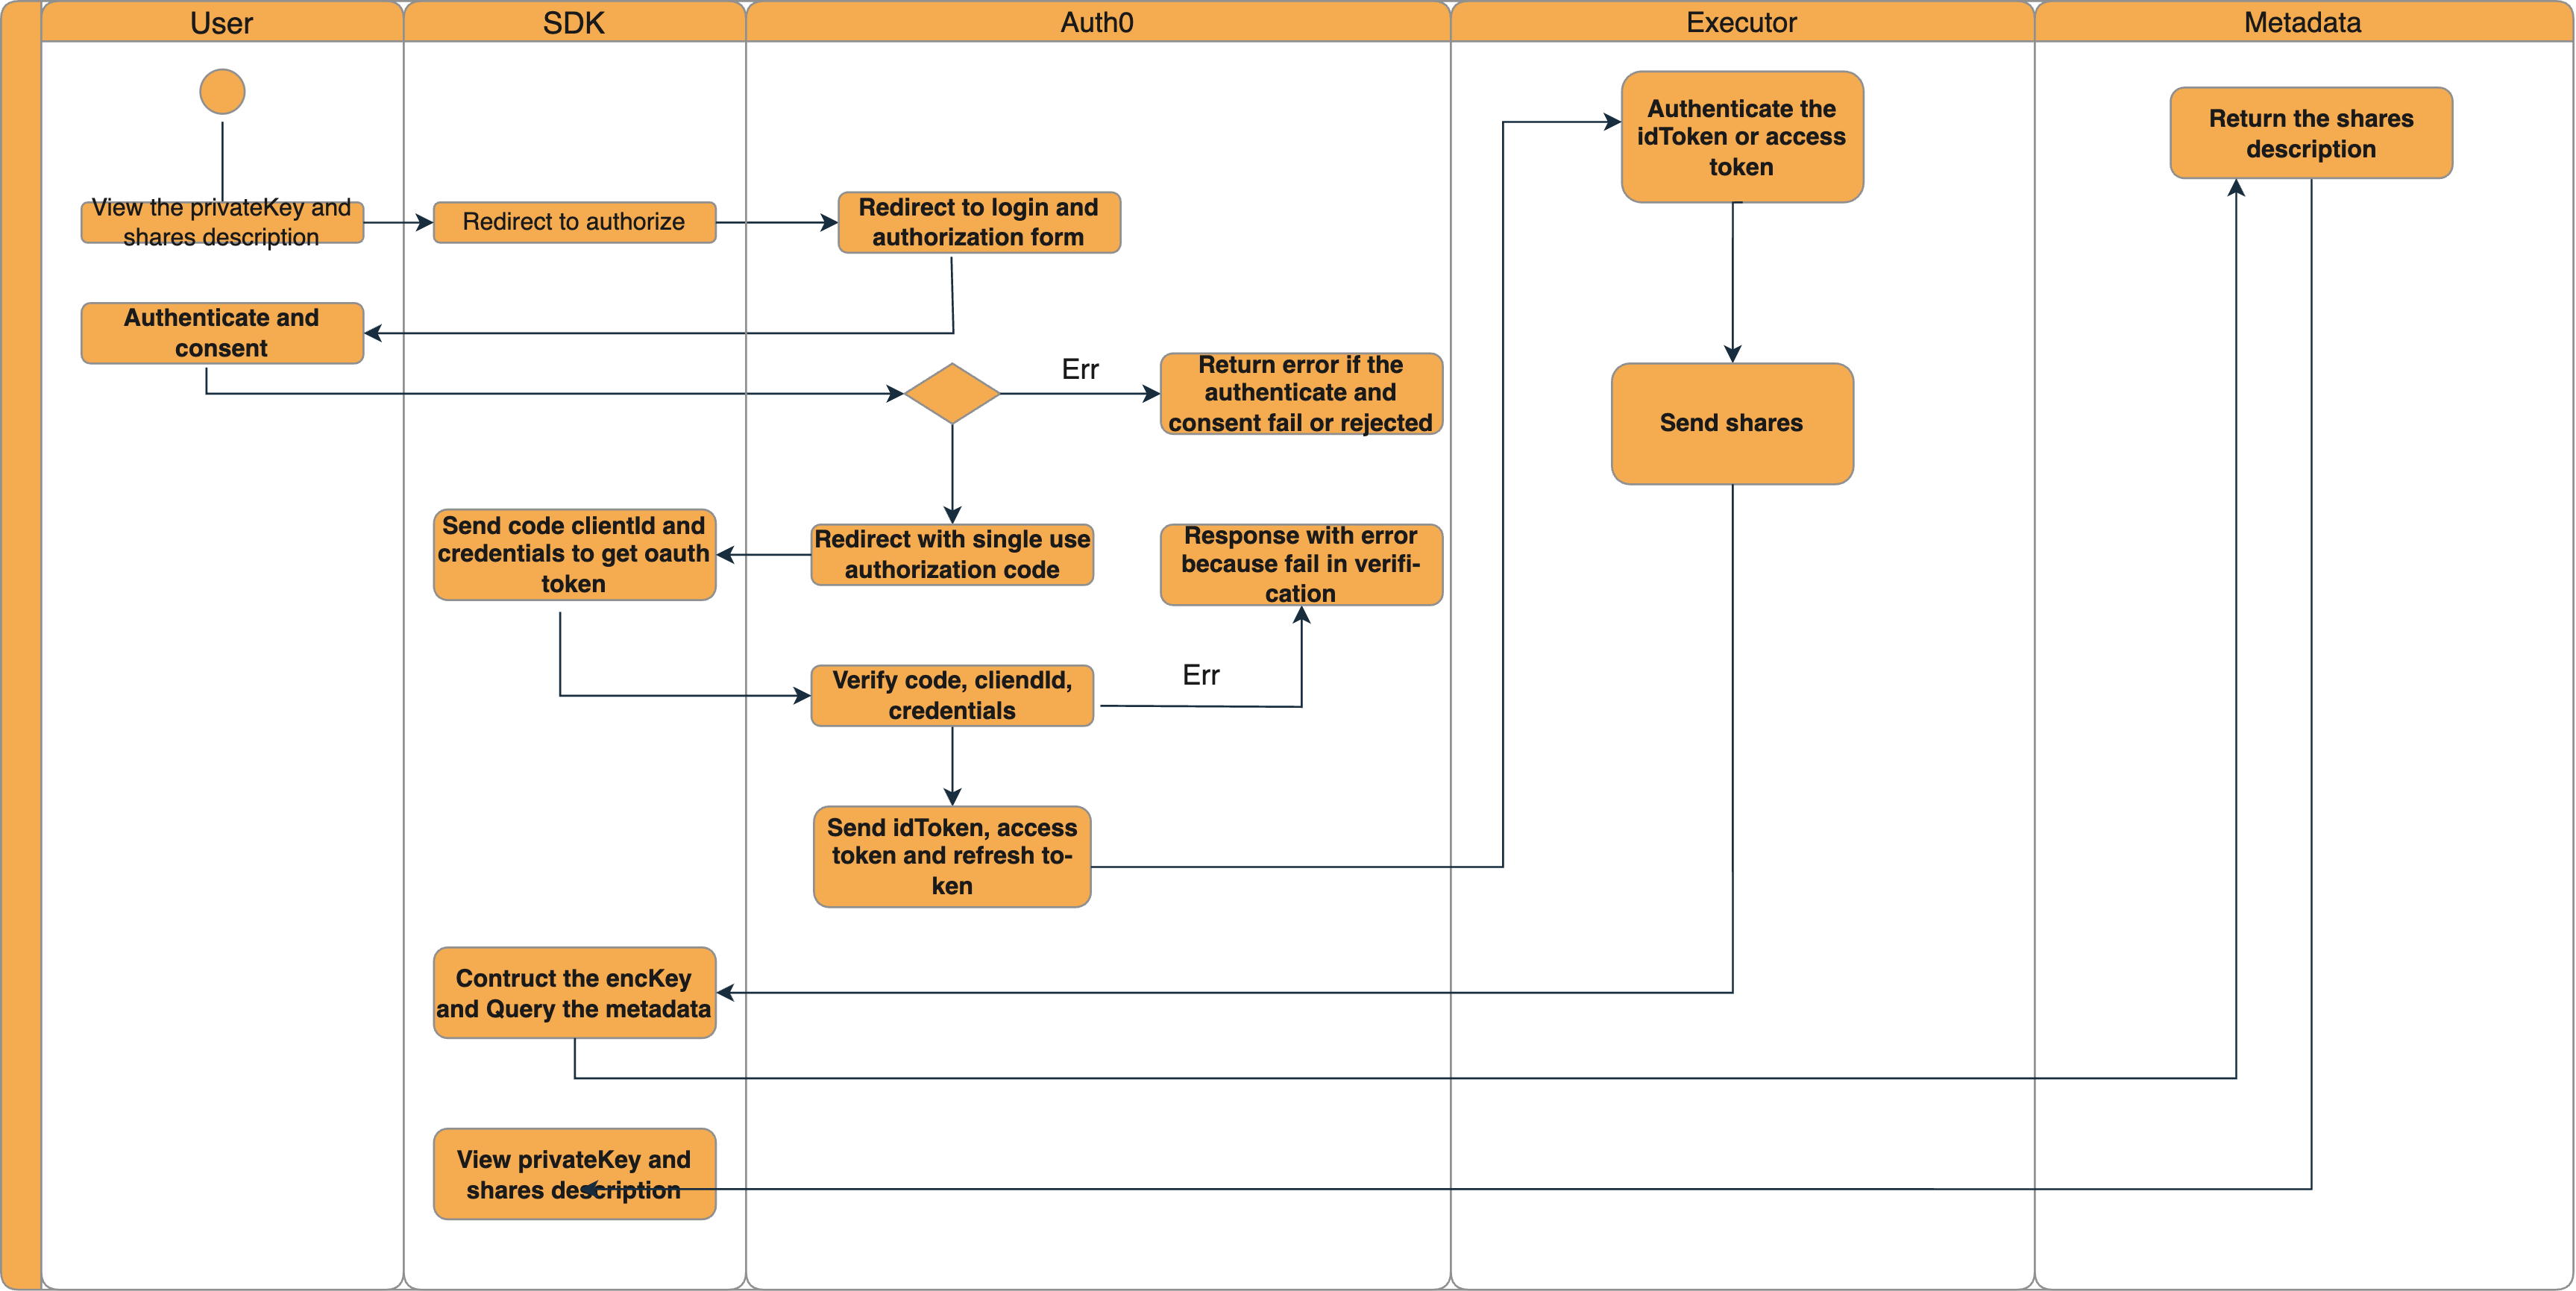
\includegraphics[scale=0.14]{Figure/view-pv-shares-activity.png}
 \caption{View private key and shares description activity}
    \label{fig:view-pv-shares-activity}
\end{figure}

The last use case, showing in \ref{fig:view-pv-shares-activity}, for the user involves viewing their private key and their shares. This functionality allows users to have full control and management over their shares, even outside the system. By providing access to their private key and the corresponding shares, users can securely store this information in a location of their choice, such as a hardware wallet or an encrypted offline storage. This feature enhances the security and flexibility of the system, as users have the freedom to manage their shares independently and ensure the safety of their cryptographic assets. Additionally, by being able to view their private key and shares, users can also perform offline verifications and audits, ensuring the integrity and accuracy of their cryptographic operations.

% Executor usecase
\begin{table}[H]
  \centering
  \begin{tabular}{|
  >{\columncolor[HTML]{32CB00}}l |lll|}
  \hline
  \textbf{Usecase code}       & \multicolumn{1}{l|}{UC001} & \multicolumn{1}{l|}{\textbf{Usecase name}} & Social login \\ \hline
  \textbf{Actor}              & \multicolumn{3}{l|}{Executor}                                                              \\ \hline
  \textbf{Pre-condition}       & \multicolumn{3}{l|}{Executor is a member of DKG}                                    \\ \hline
  \textbf{Main flow of event} & \multicolumn{3}{l|}{
            \begin{tabular}{|
              >{\columncolor[HTML]{FFFFFF}}p{2cm}|p{3cm}|p{6cm}|}
                  \hline
                  \cellcolor[HTML]{F56B00}\textbf{No} & \cellcolor[HTML]{F56B00}\textbf{Actor} & \cellcolor[HTML]{F56B00}\textbf{Action} \\ \hline
                  \textbf{1}                          & Executor                                   &  create encKey \\ \hline
                  \textbf{2}                          & Executor                                       &  Query config and number of idle keys\\ \hline
                  \textbf{3}                          & Executor                                       &  Share dealer phase\\ \hline
                  \textbf{4}                          & Smart contract                                       &  Store the commitments and shares\\ \hline
                  \textbf{5}                          & Smart contract                                     & Auto update round status\\ \hline
                  \textbf{6}                          & Excutor                                  & Query the current round status and round information\\ \hline
                  \textbf{7}                          & Executor                                   & Construct the final shares and the pubkey share from the round information\\ \hline
                  \textbf{8}                          & Executor                                   & Share row phase\\ \hline
                  \textbf{9}                          & Smart contract                                       &  Store the commitments and shares\\ \hline
                  \textbf{10}                          & Smart contract                                     & Auto update round status\\ \hline
                  \textbf{11}                          & Smart contract                                     & Push the complete round to the pool\\ \hline
            \end{tabular}
  } \\ \hline
  \textbf{Alternative flow of event} & \multicolumn{3}{l|}{
            \begin{tabular}{|
              >{\columncolor[HTML]{FFFFFF}}p{2cm}|p{3cm}|p{6cm}|}
                  \hline
                  \cellcolor[HTML]{F56B00}\textbf{No} & \cellcolor[HTML]{F56B00}\textbf{Actor} & \cellcolor[HTML]{F56B00}\textbf{Action} \\ \hline
                  \textbf{3b}                          & Executor    &  Stop and wait the next time invoking\\ \hline
            \end{tabular}
  }
  \end{tabular}
    \caption{Executor contributes in the DKG protocol}
    \label{executor-contribute-dkg}
  \end{table}
\begin{figure}[H]
 \centering
 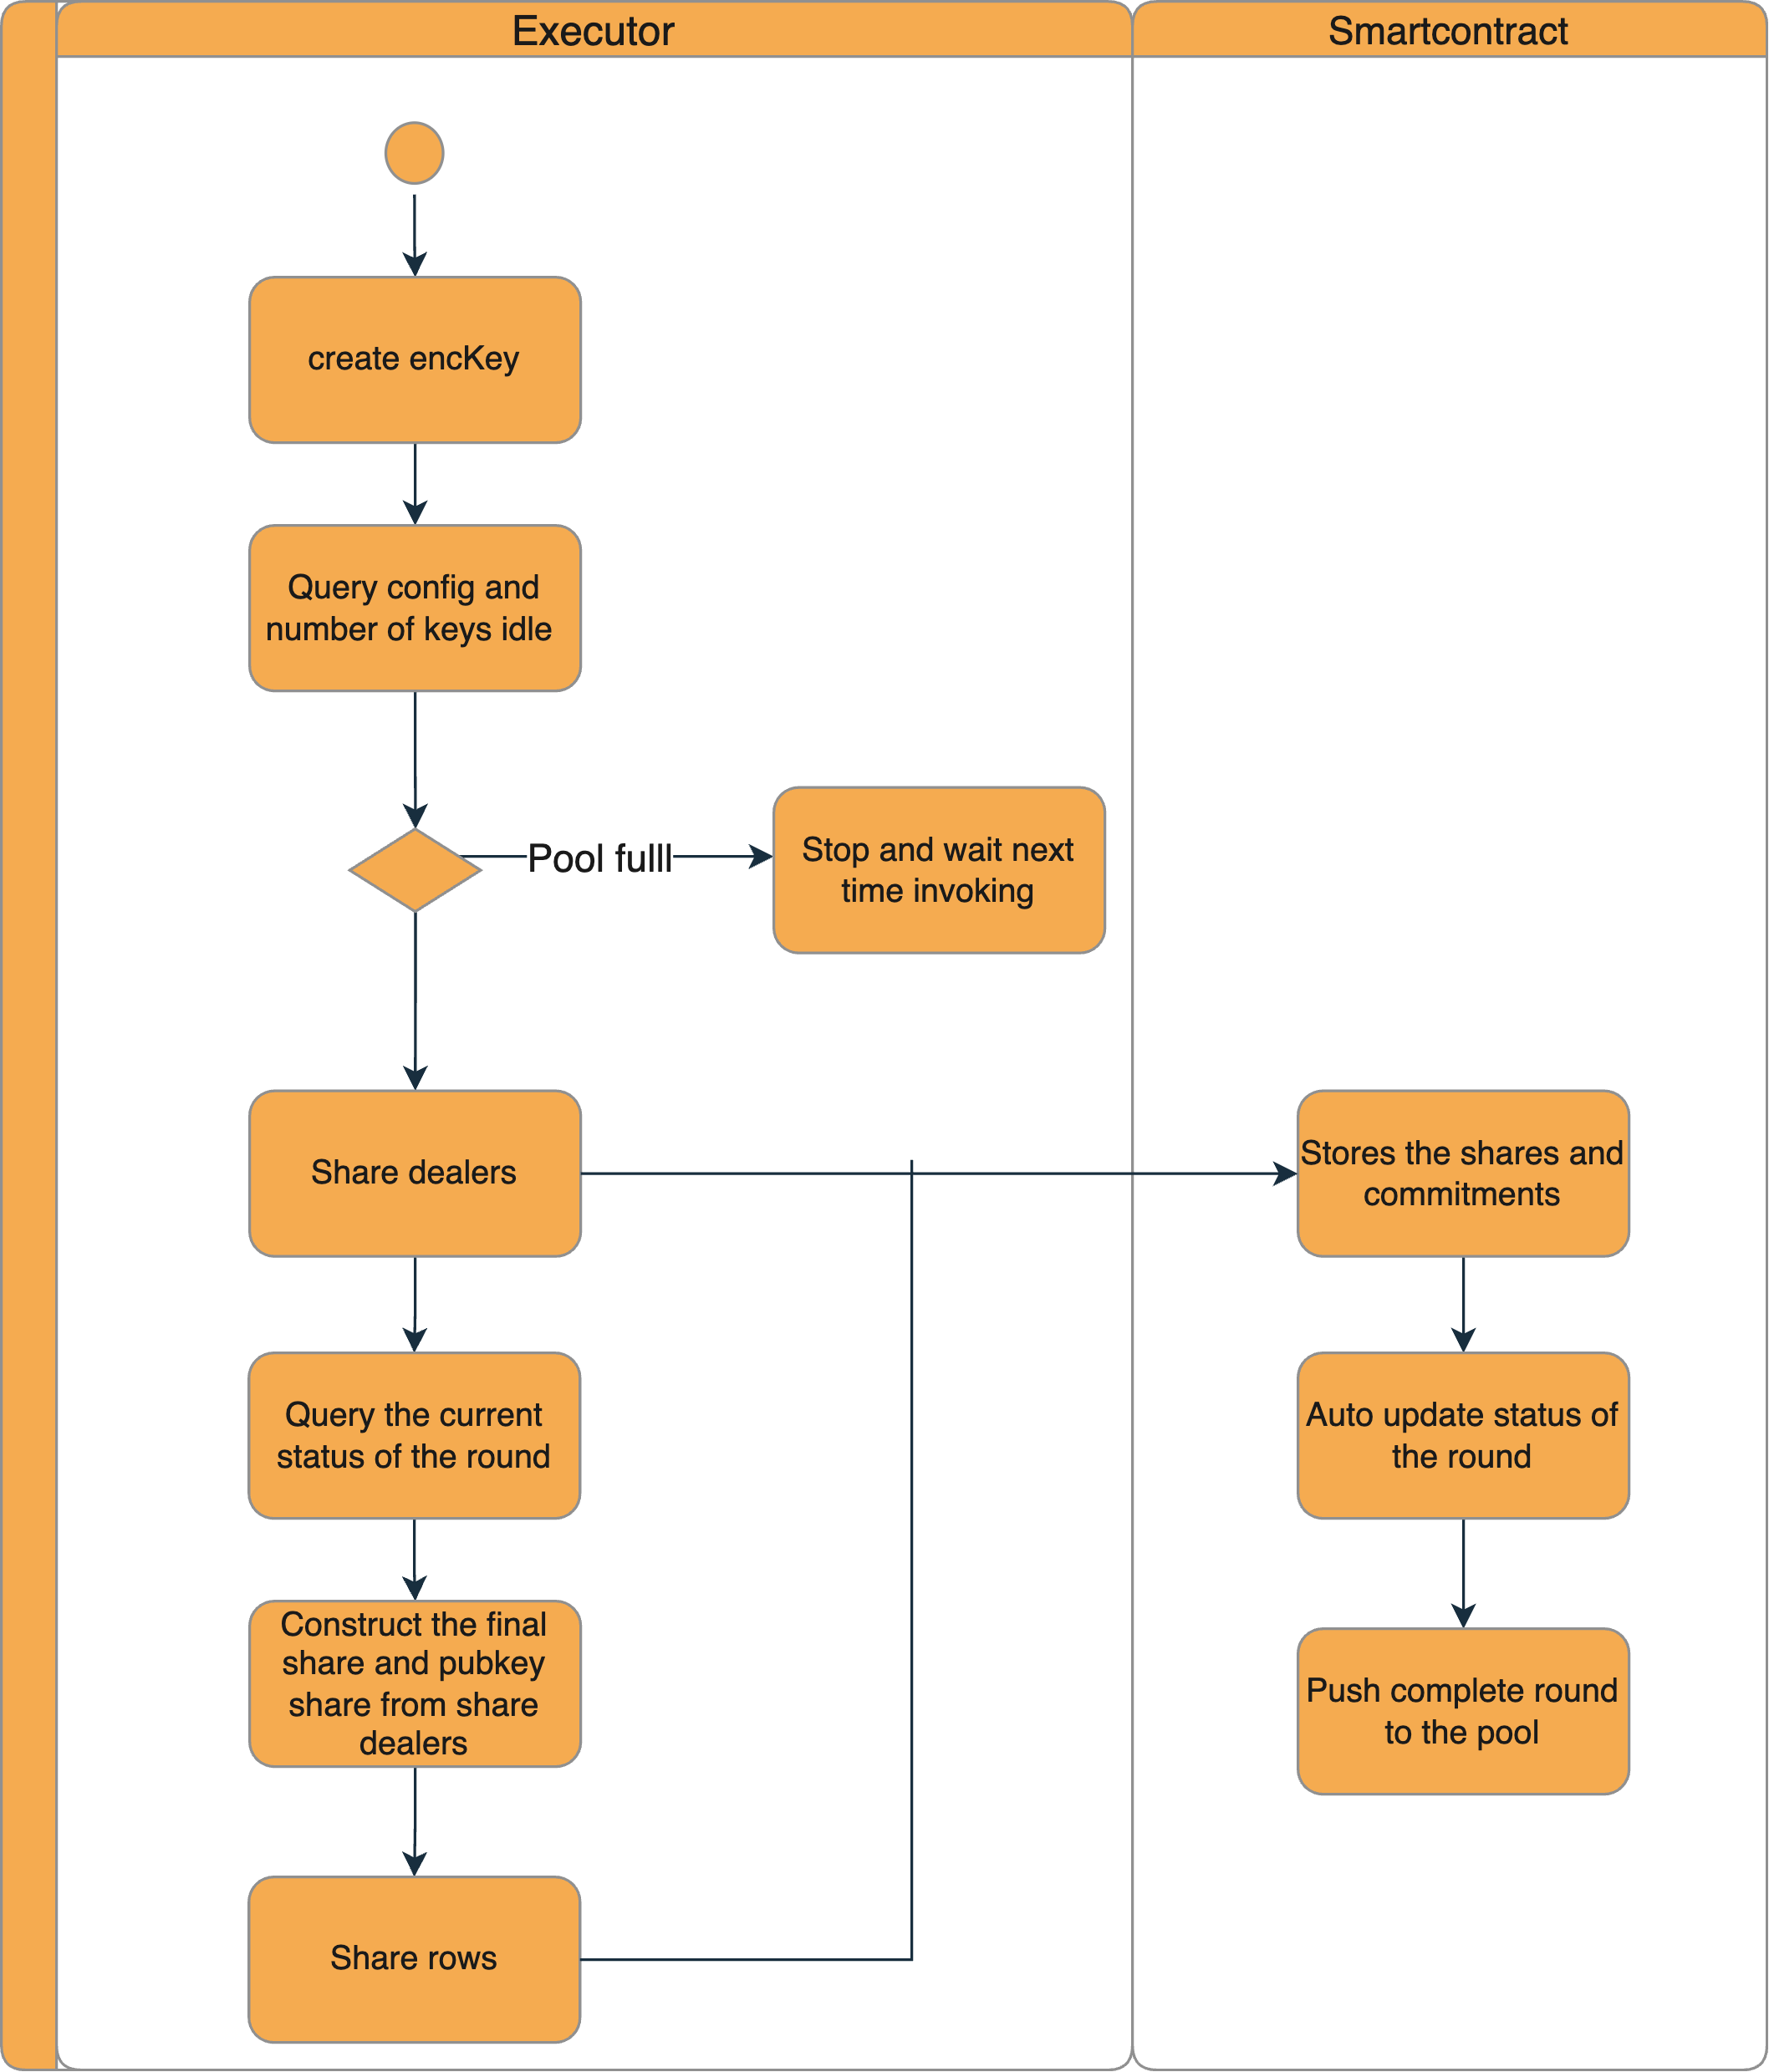
\includegraphics[scale=0.20]{Figure/executor-contribute-dkg.png}
 \caption{Executor contributes in the DKG protocol activity diagram}
    \label{fig:executor-contribute-dkg}
\end{figure}
The participation of an executor in the encKey creation procedure is crucial for the successful operation of the system. The executor, as a special actor, plays an active role in contributing to the system's functioning. The process involves multiple steps and interactions between the executor and the public smart contract deployed on the blockchain.\\
\indent Table \ref{executor-contribute-dkg} provides a comprehensive overview of the executor's involvement in the encKey creation procedure. It outlines the specific tasks and responsibilities assigned to the executor, including initiating the encKey creation round, verifying the round status, aggregating shares from other participants, generating and encrypting their own share, and finally submitting the encrypted shares to the smart contract.\\
\indent Figure \ref{fig:executor-contribute-dkg} complements the table by presenting an activity diagram that illustrates the sequence of actions performed by the executor during the encKey creation process. The diagram highlights the points of interaction between the executor and the public smart contract, depicting the flow of control and data between the two entities.


  
\begin{table}[H]
  \centering
  \begin{tabular}{|
  >{\columncolor[HTML]{32CB00}}l |lll|}
  \hline
  \textbf{Usecase code}       & \multicolumn{1}{l|}{UC001} & \multicolumn{1}{l|}{\textbf{Usecase name}} & Social login \\ \hline
  \textbf{Actor}              & \multicolumn{3}{l|}{Executor}                                                              \\ \hline
  \textbf{Pre-condition}       & \multicolumn{3}{l|}{Executor is a member of DKG}                                    \\ \hline
  \textbf{Main flow of event} & \multicolumn{3}{l|}{
            \begin{tabular}{|
              >{\columncolor[HTML]{FFFFFF}}p{2cm}|p{3cm}|p{6cm}|}
                  \hline
                  \cellcolor[HTML]{F56B00}\textbf{No} & \cellcolor[HTML]{F56B00}\textbf{Actor} & \cellcolor[HTML]{F56B00}\textbf{Action} \\ \hline
                  \textbf{1}                          & Executor                                   &  Assign key\\ \hline
                  \textbf{2}                          & Executor                                       &  Send idToken or accessToken to Auth0\\ \hline
                  \textbf{3}                          & Auth0                                       &  Verify token\\ \hline
                  \textbf{4}                          & Auth0                                       & Send verify responses\\ \hline
                  \textbf{5}                          & Executor                                       & Validate the user information\\ \hline
                  \textbf{6}                          & Executor                                  & Send the signatures for the client for aggregate\\ \hline
                  \textbf{7}                          & Executor                                   & Validate signatures\\ \hline
                  \textbf{8}                          & Executor                                   & Send request assign key with signatures to smart contract\\ \hline
                  \textbf{9}                          & Smart contract                                  & Process the request\\ \hline
            \end{tabular}
  } \\ \hline
  \textbf{Alternative flow of event} & \multicolumn{3}{l|}{
            \begin{tabular}{|
              >{\columncolor[HTML]{FFFFFF}}p{2cm}|p{3cm}|p{6cm}|}
                  \hline
                  \cellcolor[HTML]{F56B00}\textbf{No} & \cellcolor[HTML]{F56B00}\textbf{Actor} & \cellcolor[HTML]{F56B00}\textbf{Action} \\ \hline
                  \textbf{6b}                          & Executor    &  Reject request if invalid user information  \\ \hline
                  \textbf{8b}                          & Executor    &  Reject request if the valid signatures is not exceed the thresholds\\ \hline
            \end{tabular}
  }
  \end{tabular}
    \caption{Executor assigns key}
    \label{executor-assign-key}
  \end{table}
\begin{figure}[H]
 \centering
 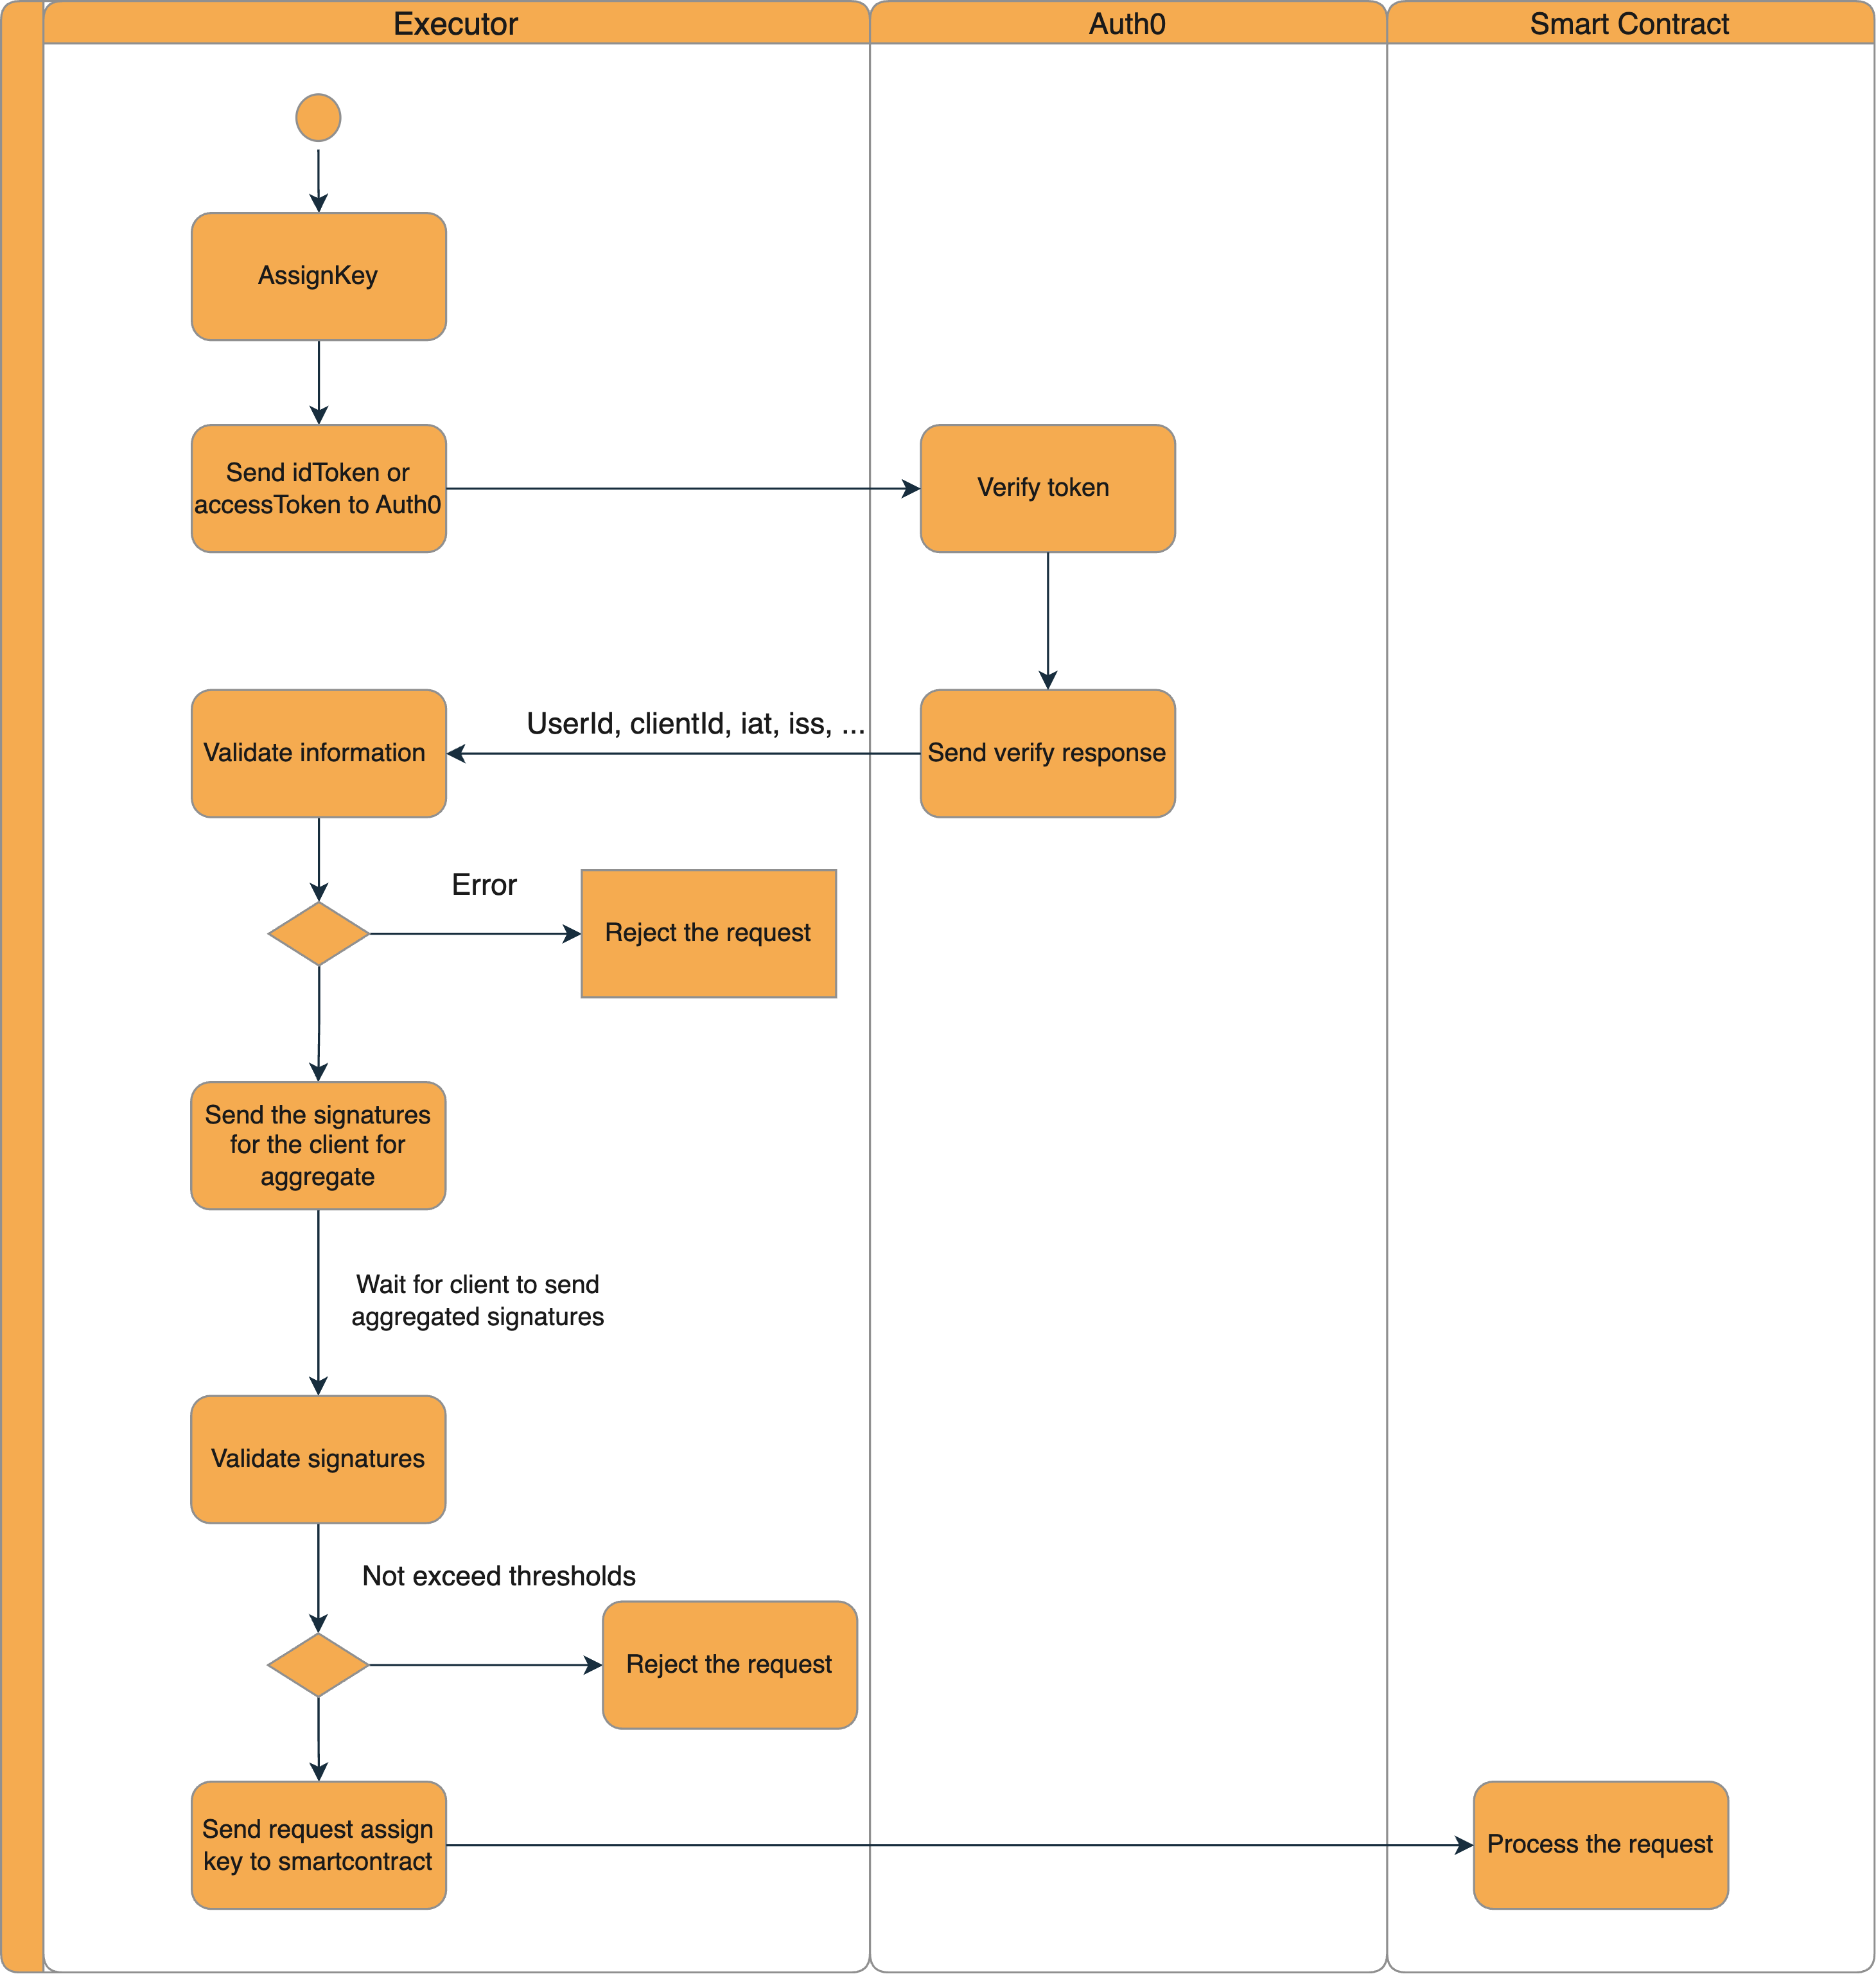
\includegraphics[scale=0.14]{Figure/executor-assign-key.png}
 \caption{View private key and shares description activity}
    \label{fig:executor-assign-key}
\end{figure}
Figure \ref{fig:executor-assign-key} provides a detailed illustration of the process in which an executor assigns an encKey to a user in the social login system for Web3. This diagram showcases the interactions between three key components: Auth0, the smart contract, and the executor.

\section{Technologies}
In addition to the blockchain technology, smart contracts, and oracles described in the background section, I would like to describe other system-building tools and libraries.

\subsection{Backend}
\subsubsection{ExpressJs}
Express.js is a well-known web application framework for Node.js that facilitates the construction of scalable and robust web applications. It offers a minimalistic and adaptable approach to web development, making it simple for developers to construct server-side applications.\\
\indent One of the primary benefits of Express.js is its simplicity and usability. It provides developers with a framework that is minimal and agnostic, allowing them to structure their applications according to their needs. Express.js adheres to a middleware-based architecture, enabling developers to easily incorporate middleware components to handle various application aspects, such as routing, request processing, and error handling.\\
\indent Express.js \cite{expressjs} is widely recognized for its robust routing capabilities. It offers a concise and straightforward syntax for defining routes and managing various HTTP methods, including GET, POST, PUT, and DELETE. Express.js makes it simple to define routes for handling incoming requests and performing operations such as retrieving data from a database, processing the data, and returning the appropriate response to the client.\\
\indent Within the system architecture, Express.js serves as a robust and versatile server framework that plays a vital role in handling the requests associated with the metadata of the system. Leveraging the power of Express.js, the backend of the system is equipped with the capability to receive, process, and respond to various types of requests related to the metadata.
Overall, the utilization of Express.js as the server framework for handling metadata requests empowers the system to efficiently manage and process metadata-related operations. Its robust routing system, extensible middleware ecosystem, and high-performance nature make Express.js an ideal choice for building scalable and reliable backend systems that handle metadata effectively.

\subsubsection{JSON-RPC and Jayson library}
JSON-RPC\cite{jsonrpc} is a remote procedure call protocol encoded in JSON. It allows for the execution of remote procedures on a server and the exchange of structured data between the client and the server. In the system, JSON-RPC is employed to facilitate communication between different components and services, enabling the invocation of remote procedures and the transmission of data in a standardized and efficient manner. The utilization of JSON-RPC ensures interoperability and seamless integration between various system components.\\
\indent The Jayson library, a JSON-RPC implementation for Node.js, is used to manage JSON-RPC communication between the client and server. Jayson is a framework for creating JSON-RPC servers and clients in Node.js that is lightweight and efficient. It simplifies the creation and management of JSON-RPC requests and responses, facilitating integration with the server and client components of the system. You can define the server-side methods that will be exposed to clients via JSON-RPC using Jayson. Jayson handles the serialization and deserialization of JSON-RPC messages. These methods can be implemented as functions or class methods. It offers a convenient API for managing the request payload, extracting the method name and parameters, and executing the appropriate server-side logic. The Jayson library integrates seamlessly with the Express.js server, allowing the server component of the system to process incoming JSON-RPC requests using the specified server-side methods. It offers an elegant and efficient solution for implementing JSON-RPC communication in Node.js, making it an excellent choice for the communication layer of the system.\\
\indent The Jayson library is incorporated in the system to process JSON-RPC requests from the client to the executor component. This decision is made because the role of the executor predominantly entails handling and processing requests unrelated to database operations. Using Jayson for JSON-RPC communication allows the executor to efficiently manage requests without requiring direct database interaction. JSON-RPC requests may include information and instructions for the executor to perform particular duties or computations, such as generating shares, decrypting data, or validating signatures. The executor processes these requests, carries out the required logic, and returns the appropriate response to the client. Implementing JSON-RPC for the executor enables a clean separation of concerns, as the executor component is exclusively focused on executing the requested tasks and does not interact directly with the databases. This design decision streamlines the executor's responsibilities and improves its capacity to respond to client requests. Using a well-established library such as Jayson also facilitates the implementation of JSON-RPC communication, resulting in a robust and dependable solution. The library manages the serialization and deserialization of JSON-RPC messages, ensuring that requests and responses are formatted correctly and are compatible between the client and executor. This simplifiees the development process and helps keep the communication protocol consistent and compatible.
\subsection{Database}
MySQL\cite{mysql} is an extensively utilized open-source relational database management system (RDBMS) for storing and querying structured data. In your system, MySQL is used exclusively for storing and querying metadata in the metadata backend section. MySQL offers a dependable and effective method for storing structured data in tables, with support for a variety of data types and indexing options. It provides comprehensive transactional capabilities, ensuring data consistency and integrity during concurrent operations. MySQL's robust query language, SQL (Structured Query Language), enables efficient data retrieval and manipulation through a variety of query operations, including filtering, sorting, joining, and aggregating. The metadata backend section of the system is responsible for managing and storing metadata associated with user authentication, authorization, and other pertinent data. MySQL functions as the underlying database technology for the structured storage of this metadata. In the future, the metadata may include encrypted shares or ecrypted information of multiple system modules. By leveraging MySQL, the system can take advantage of its scalability and performance enhancements, enabling it to efficiently manage large volumes of metadata. In addition, MySQL provides security mechanisms, data backup and recovery, and replication options, all of which contribute to the dependability and accessibility of your metadata storage. 
\subsection{Frontend}
The frontend of the system plays a critical role as it enables users or clients to interact with the system in a seamless and user-friendly manner. It serves as the interface through which users can access the system's features, functionalities, and data.\\

\textbf{Tkey} is a GitHub-hosted open-source library designed to provide cryptographic key management capabilities. The library seeks to simplify the handling and management of cryptographic keys, making it easier for application developers to implement robust security measures. The Tkey library provides a vast array of key generation, storage, and usage-related features and functions. It supports a variety of cryptographic algorithms, such as symmetric and asymmetric encryption, digital signatures, and hash functions. This enables developers to employ various cryptographic techniques based on their particular requirements. Tkey's emphasis on security is one of its primary features. The library employs key management best practices, such as secure key storage, protection against unauthorized access, and secure key sharing protocols. Tkey adheres to industry standards and recommendations to assure the privacy, integrity, and accessibility of cryptographic keys. In addition, Tkey provides a simple and intuitive API, easing the integration of cryptographic key management into applications. The library provides developers with comprehensive documentation and implementation examples.
\indent Based on the foundation provided by the Tkey open-source library, our system extends its functionality by implementing modules that are specifically tailored to our application's needs. These custom modules enhance Tkey's compatibility with our system's architecture by enhancing its primary features.
\subsection{Virtualization}
Docker is an open-source platform that has revolutionized the way applications are developed, shipped, and deployed. It provides developers with a powerful set of tools to automate the packaging and deployment of applications inside lightweight, portable containers. By leveraging containerization technology, Docker enables the creation of isolated environments that encapsulate an application and its dependencies. This ensures that the application runs consistently and predictably across different systems, regardless of the underlying infrastructure.\\
\indent Containers are self-contained units that contain everything needed to run an application, including the code, runtime, system tools, and libraries. They offer advantages such as isolation, scalability, and reproducibility. With Docker, developers can package their applications along with all the necessary dependencies into a container image, which can then be deployed on any system that has Docker installed. This eliminates the need for complex setup processes and reduces compatibility issues between different environments.\\
\indent Docker Compose is a complementary tool to Docker that simplifies the management of multi-container applications. It allows developers to define and configure multiple containers, their networks, and volumes using a simple YAML file. This makes it easier to define complex, interconnected services and orchestrate their deployment. With Docker Compose, developers can quickly spin up an entire application stack with a single command, making the development and testing process more efficient.\\
\indent In the context of this thesis, Docker plays a crucial role in encapsulating the application and its dependencies, ensuring portability and consistency. By using Docker, the application can be packaged into a container image, making it highly portable and enabling easy deployment across different environments. Docker-compose is utilized during the development phase to define and manage the various services and dependencies required by the application. This allows for rapid system configuration and simplifies the process of setting up a development environment.
\subsection{Rust, wasm and cosmwasm}
Rust is a systems programming language known for its emphasis on performance, reliability, and safety. It offers a high level of control over system resources while providing memory safety guarantees through its ownership and borrowing system. Rust's combination of low-level control and high-level abstractions makes it well-suited for building efficient and secure software, including blockchain applications.\\
\indent WebAssembly (Wasm) is a binary instruction format that allows for the execution of code on a variety of platforms, including web browsers. It provides a portable and efficient runtime environment for running code at near-native speeds. Rust is one of the languages that can compile to WebAssembly, allowing developers to leverage Rust's performance and safety features in web-based applications.\\
\indent CosmWasm is a specific implementation of WebAssembly designed for smart contract development within the Cosmos ecosystem. It extends the capabilities of WebAssembly to support the unique requirements of blockchain-based smart contracts. With CosmWasm, developers can write smart contracts in Rust and compile them to WebAssembly, leveraging the language's safety guarantees and performance optimizations. CosmWasm provides a secure execution environment for these smart contracts, ensuring the integrity and correctness of their execution on the blockchain.\\
\indent The combination of Rust, WebAssembly, and CosmWasm offers several benefits for blockchain development. Rust's memory safety features help mitigate vulnerabilities and potential exploits in smart contracts, reducing the risk of security breaches. WebAssembly enables efficient execution of the compiled Rust code across different platforms, allowing for interoperability and portability. CosmWasm, as an implementation of WebAssembly tailored for blockchain smart contracts, provides a secure and optimized environment for executing Rust-based smart contracts within the Cosmos ecosystem.\\

\section{Diagram design}
\subsection{Sequence diagram}
\begin{figure}[H]
 \centering
 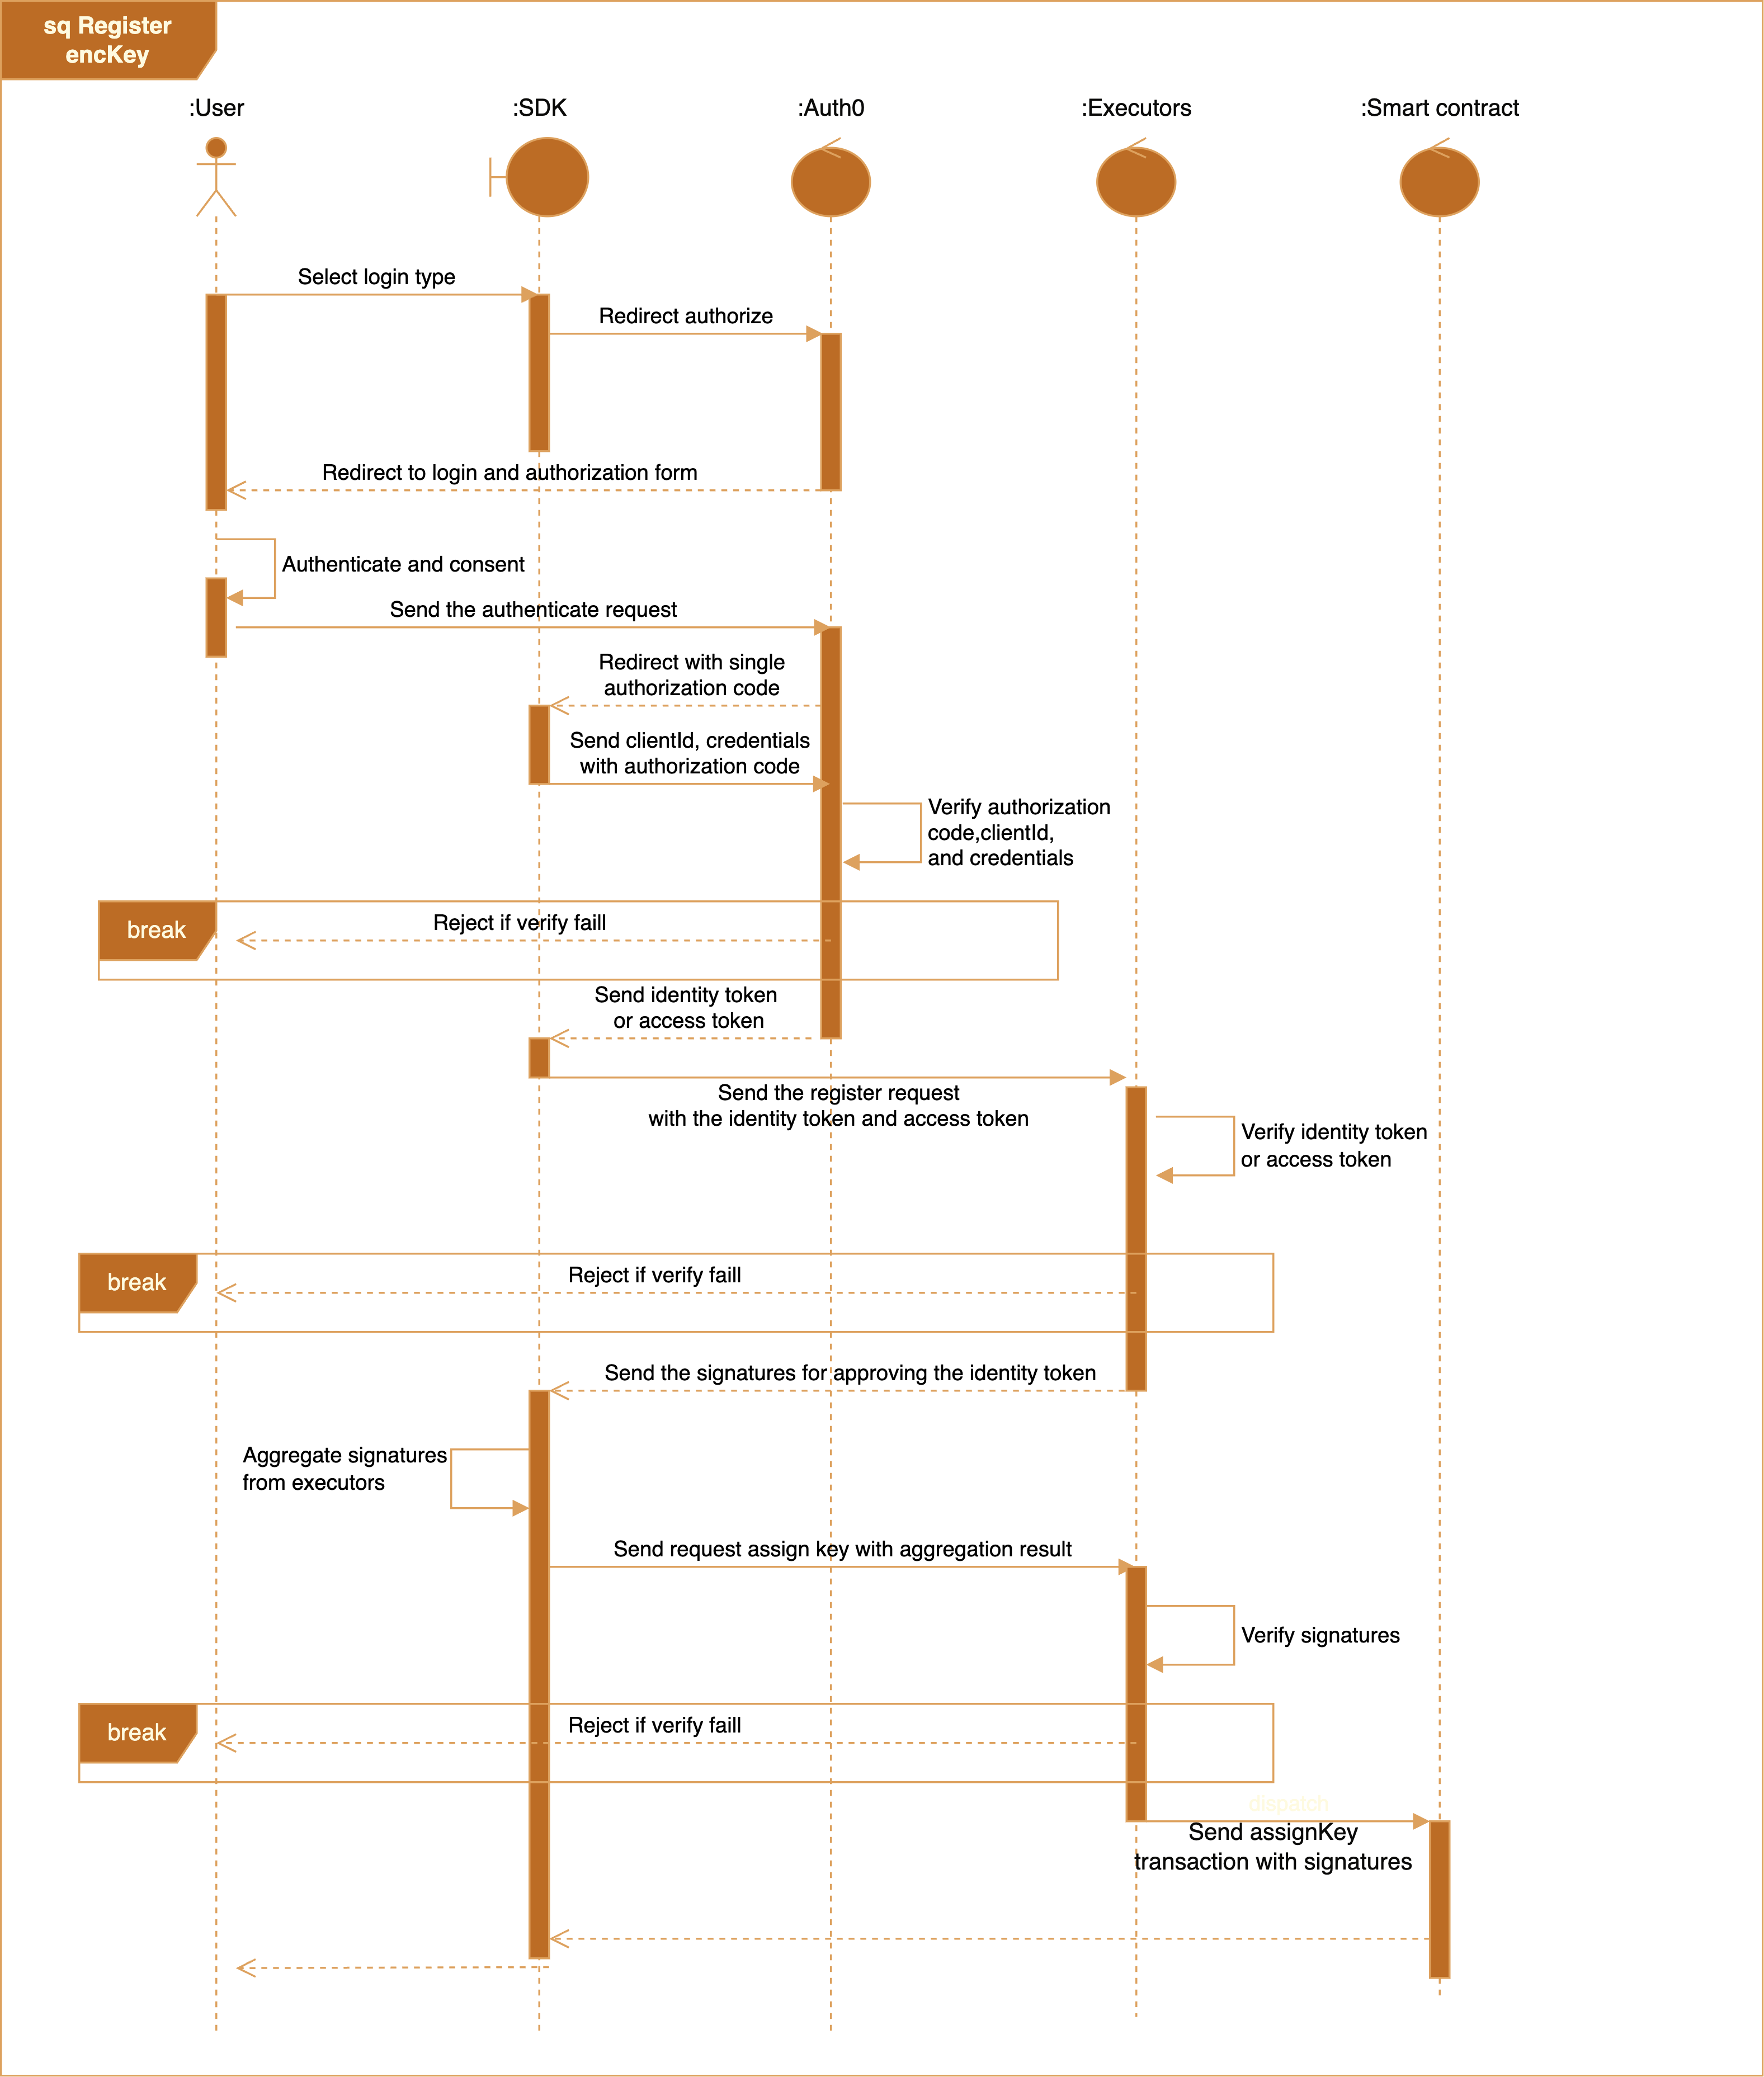
\includegraphics[scale=0.14]{Figure/register-sequence-diagram.png}
 \caption{Register sequence diagram}
    \label{fig:register-sequence-diagram}
\end{figure}
The diagram \ref{fig:register-sequence-diagram} depicts the registration procedure for a new encKey.  The user must select the social registration type and successfully complete the validation procedure.
\begin{figure}[H]
 \centering
 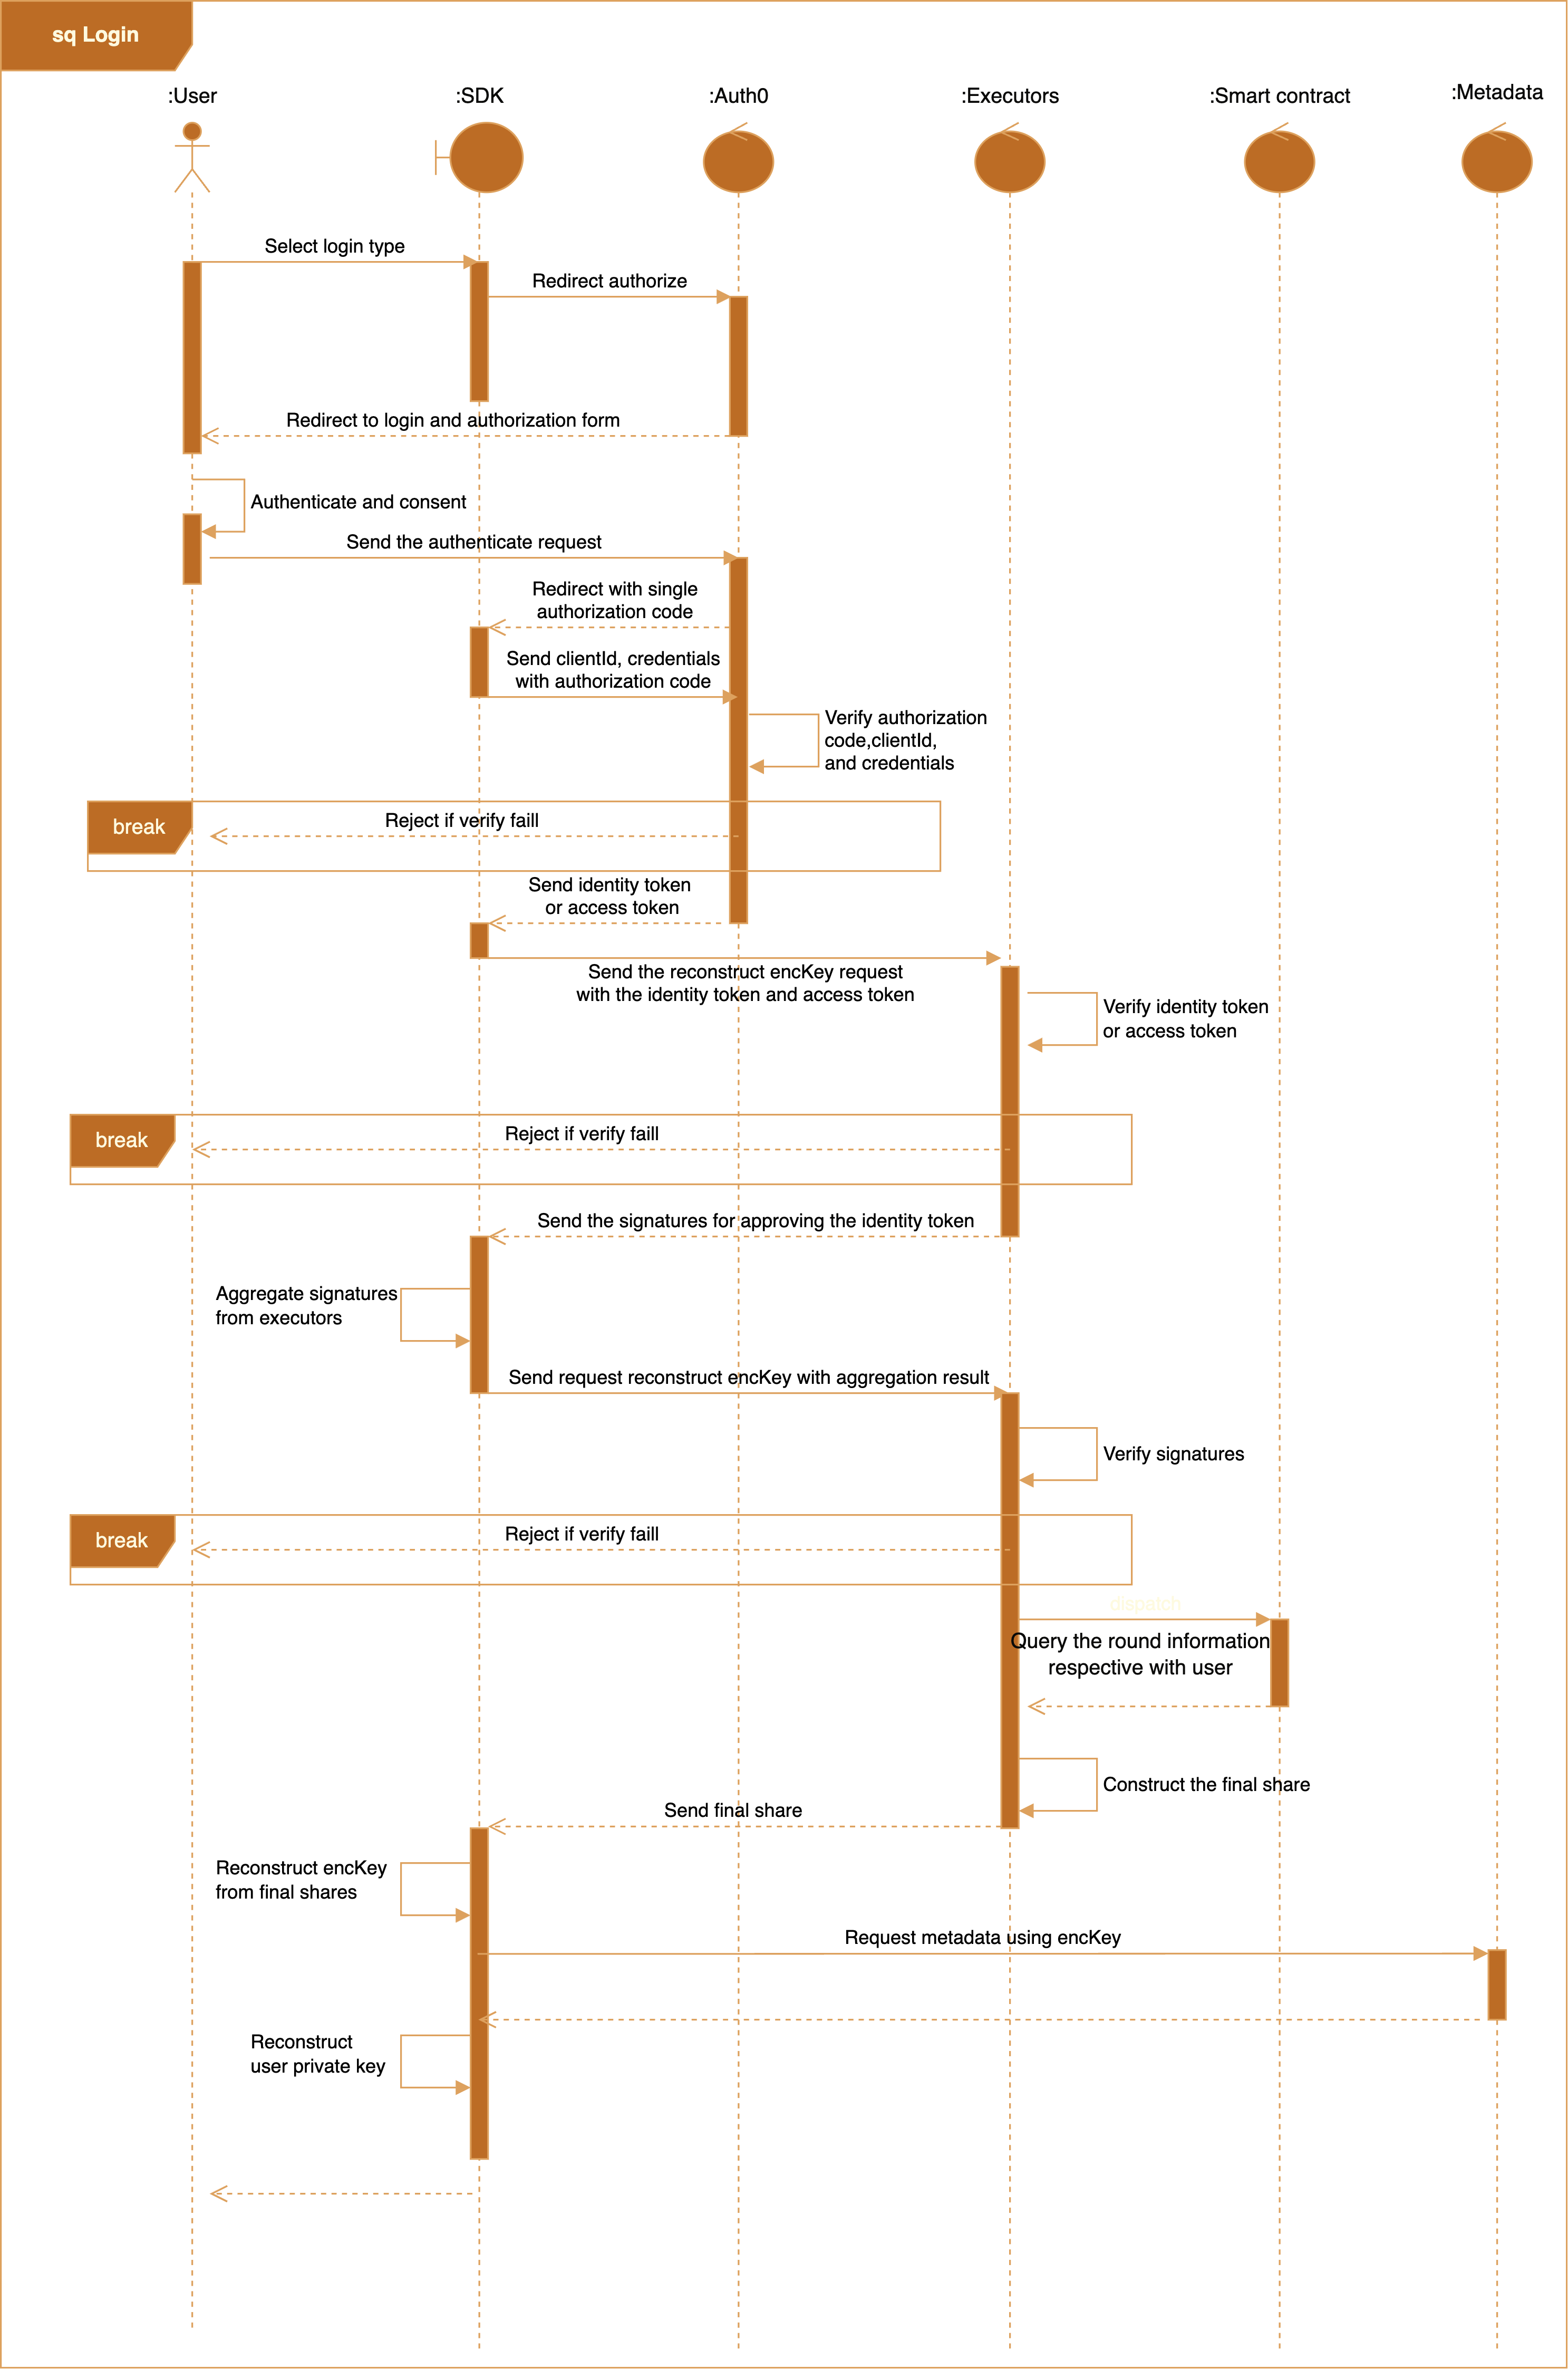
\includegraphics[scale=0.14]{Figure/login-sequence-diagram.png}
 \caption{Login sequence diagram}
    \label{fig:Login-sequence-diagram}
\end{figure}
The diagram \ref{fig:Login-sequence-diagram} depicts the social authentication system's sign-in procedure. This procedure describes how the user's data pass validation and how the user reconstructs their private key.
\begin{figure}[H]
 \centering
 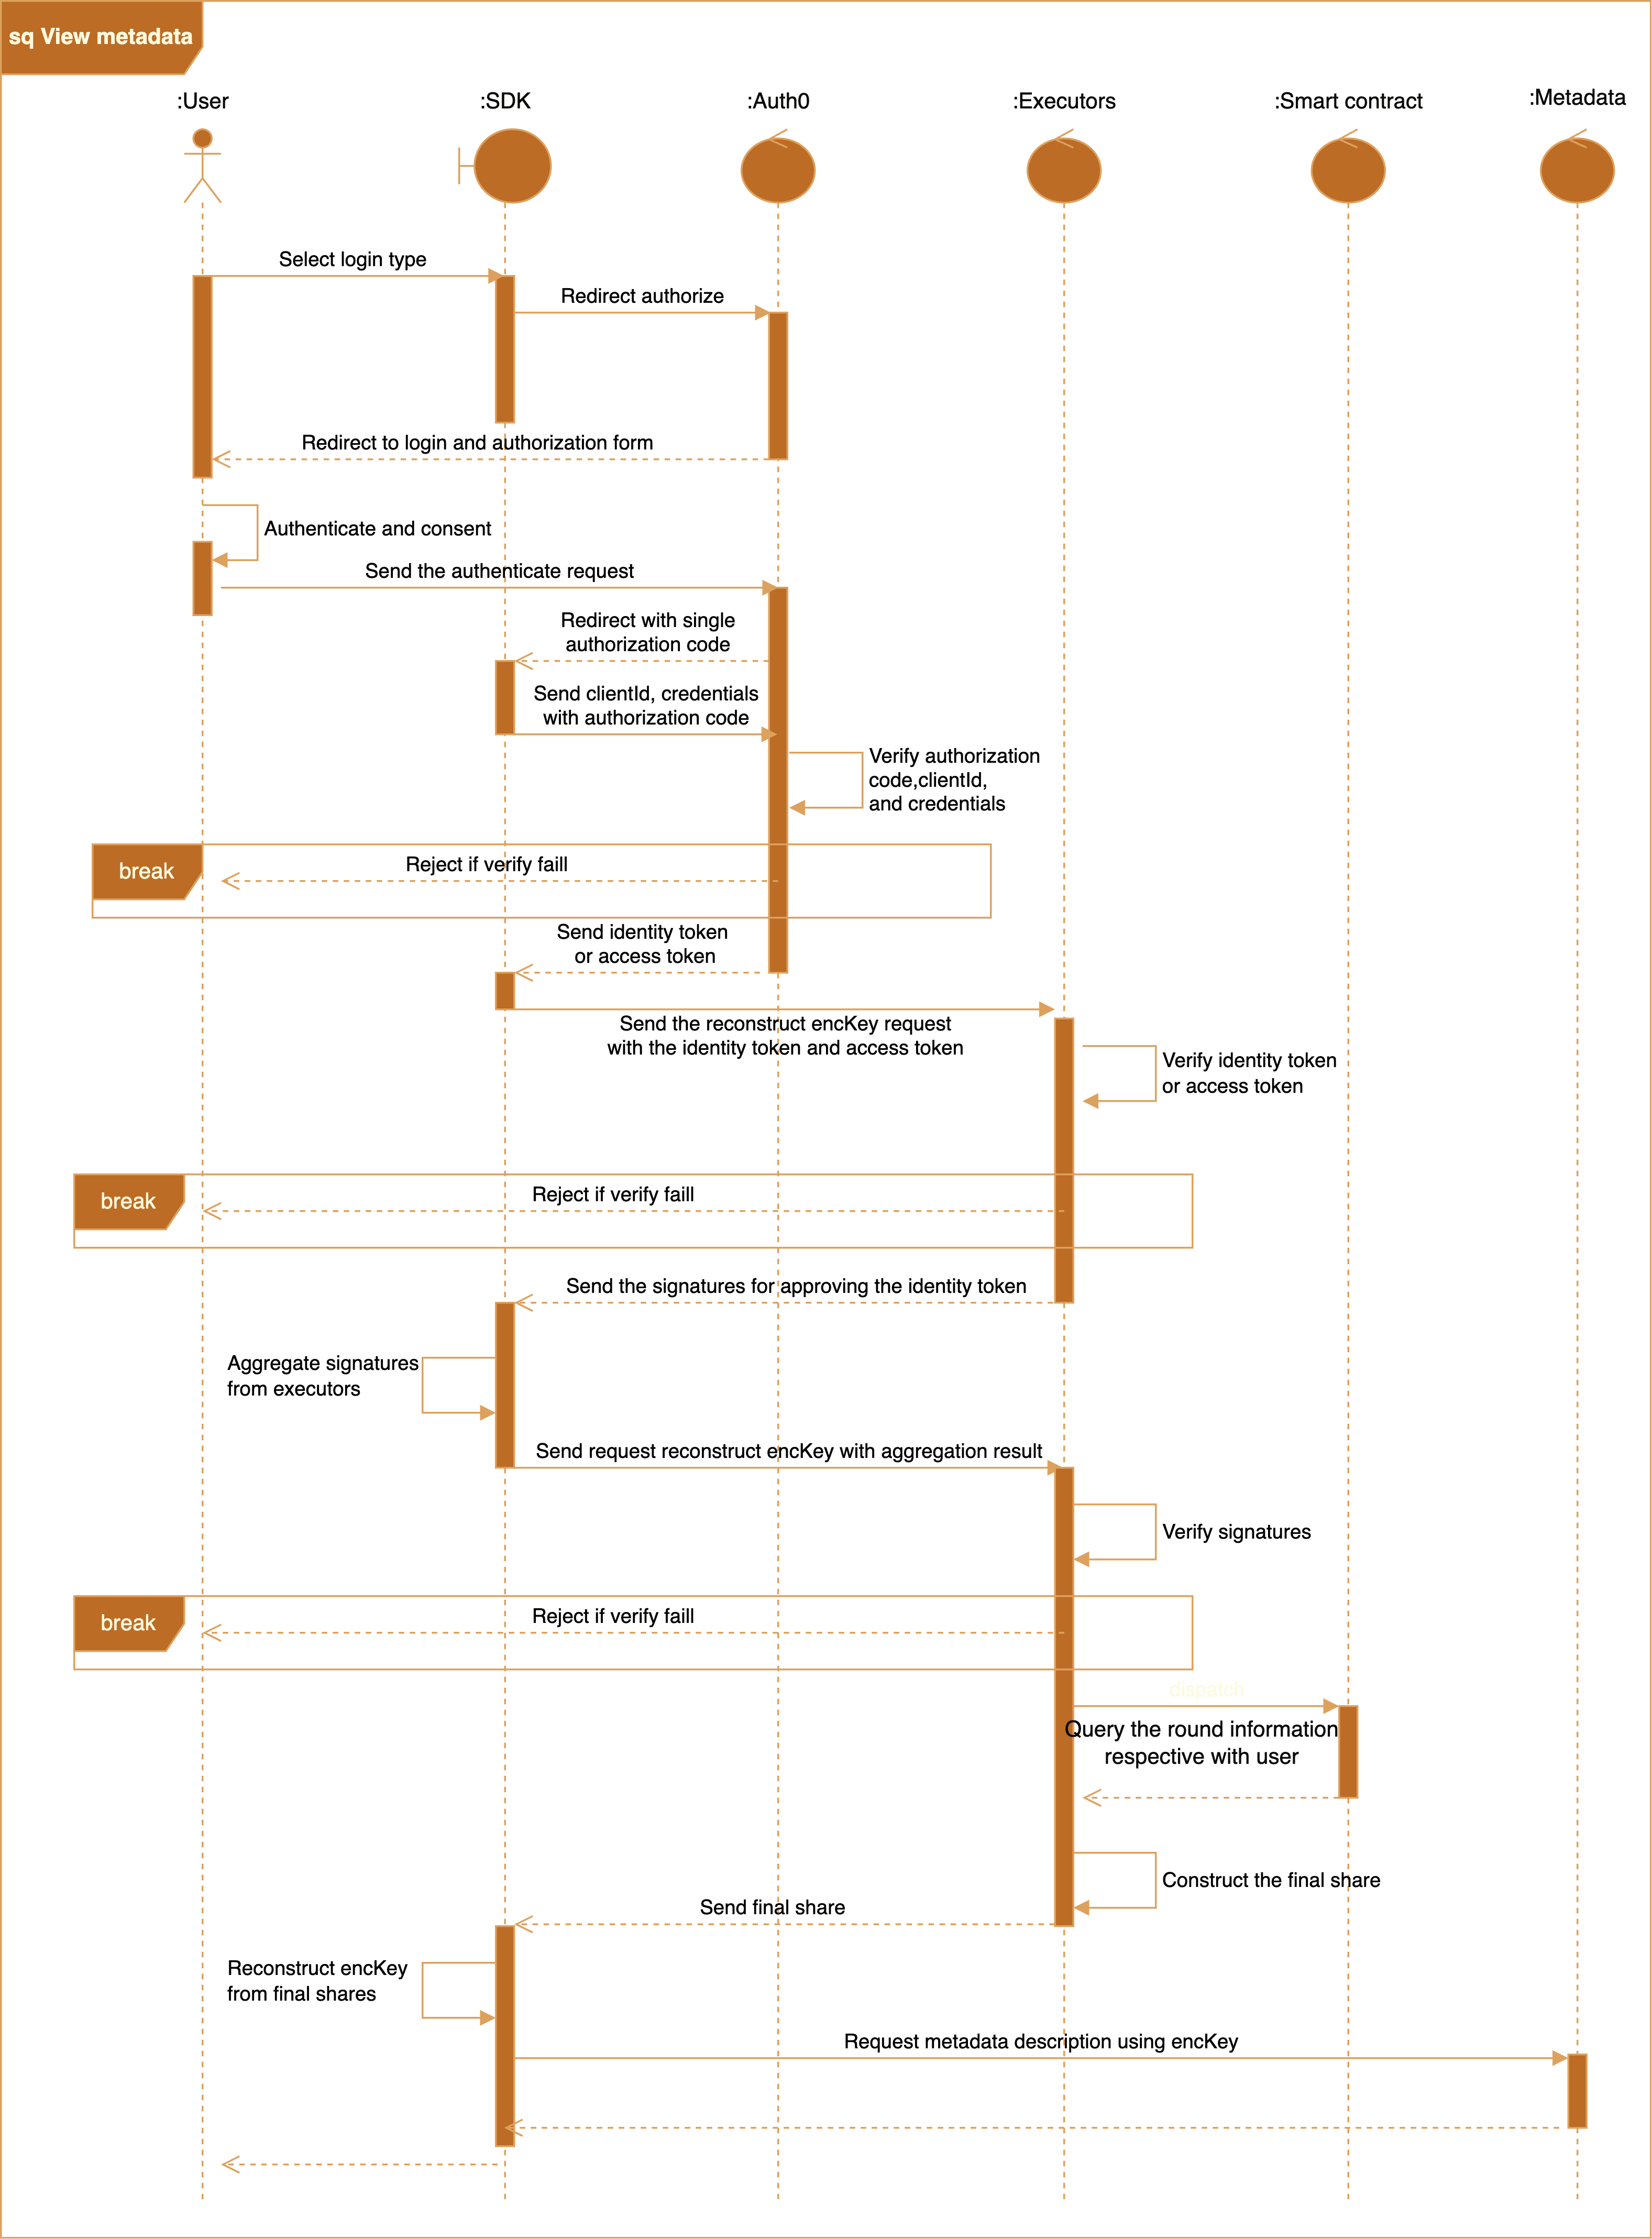
\includegraphics[scale=0.14]{Figure/view-sequence-diagram.png}
 \caption{View share description sequence diagram}
    \label{fig:view-sequence-diagram}
\end{figure}
After logging into the system, users desire to view their share descriptions and private keys. This procedure is depicted graphically in the diagram \ref{fig:view-sequence-diagram}.
\begin{figure}[H]
 \centering
 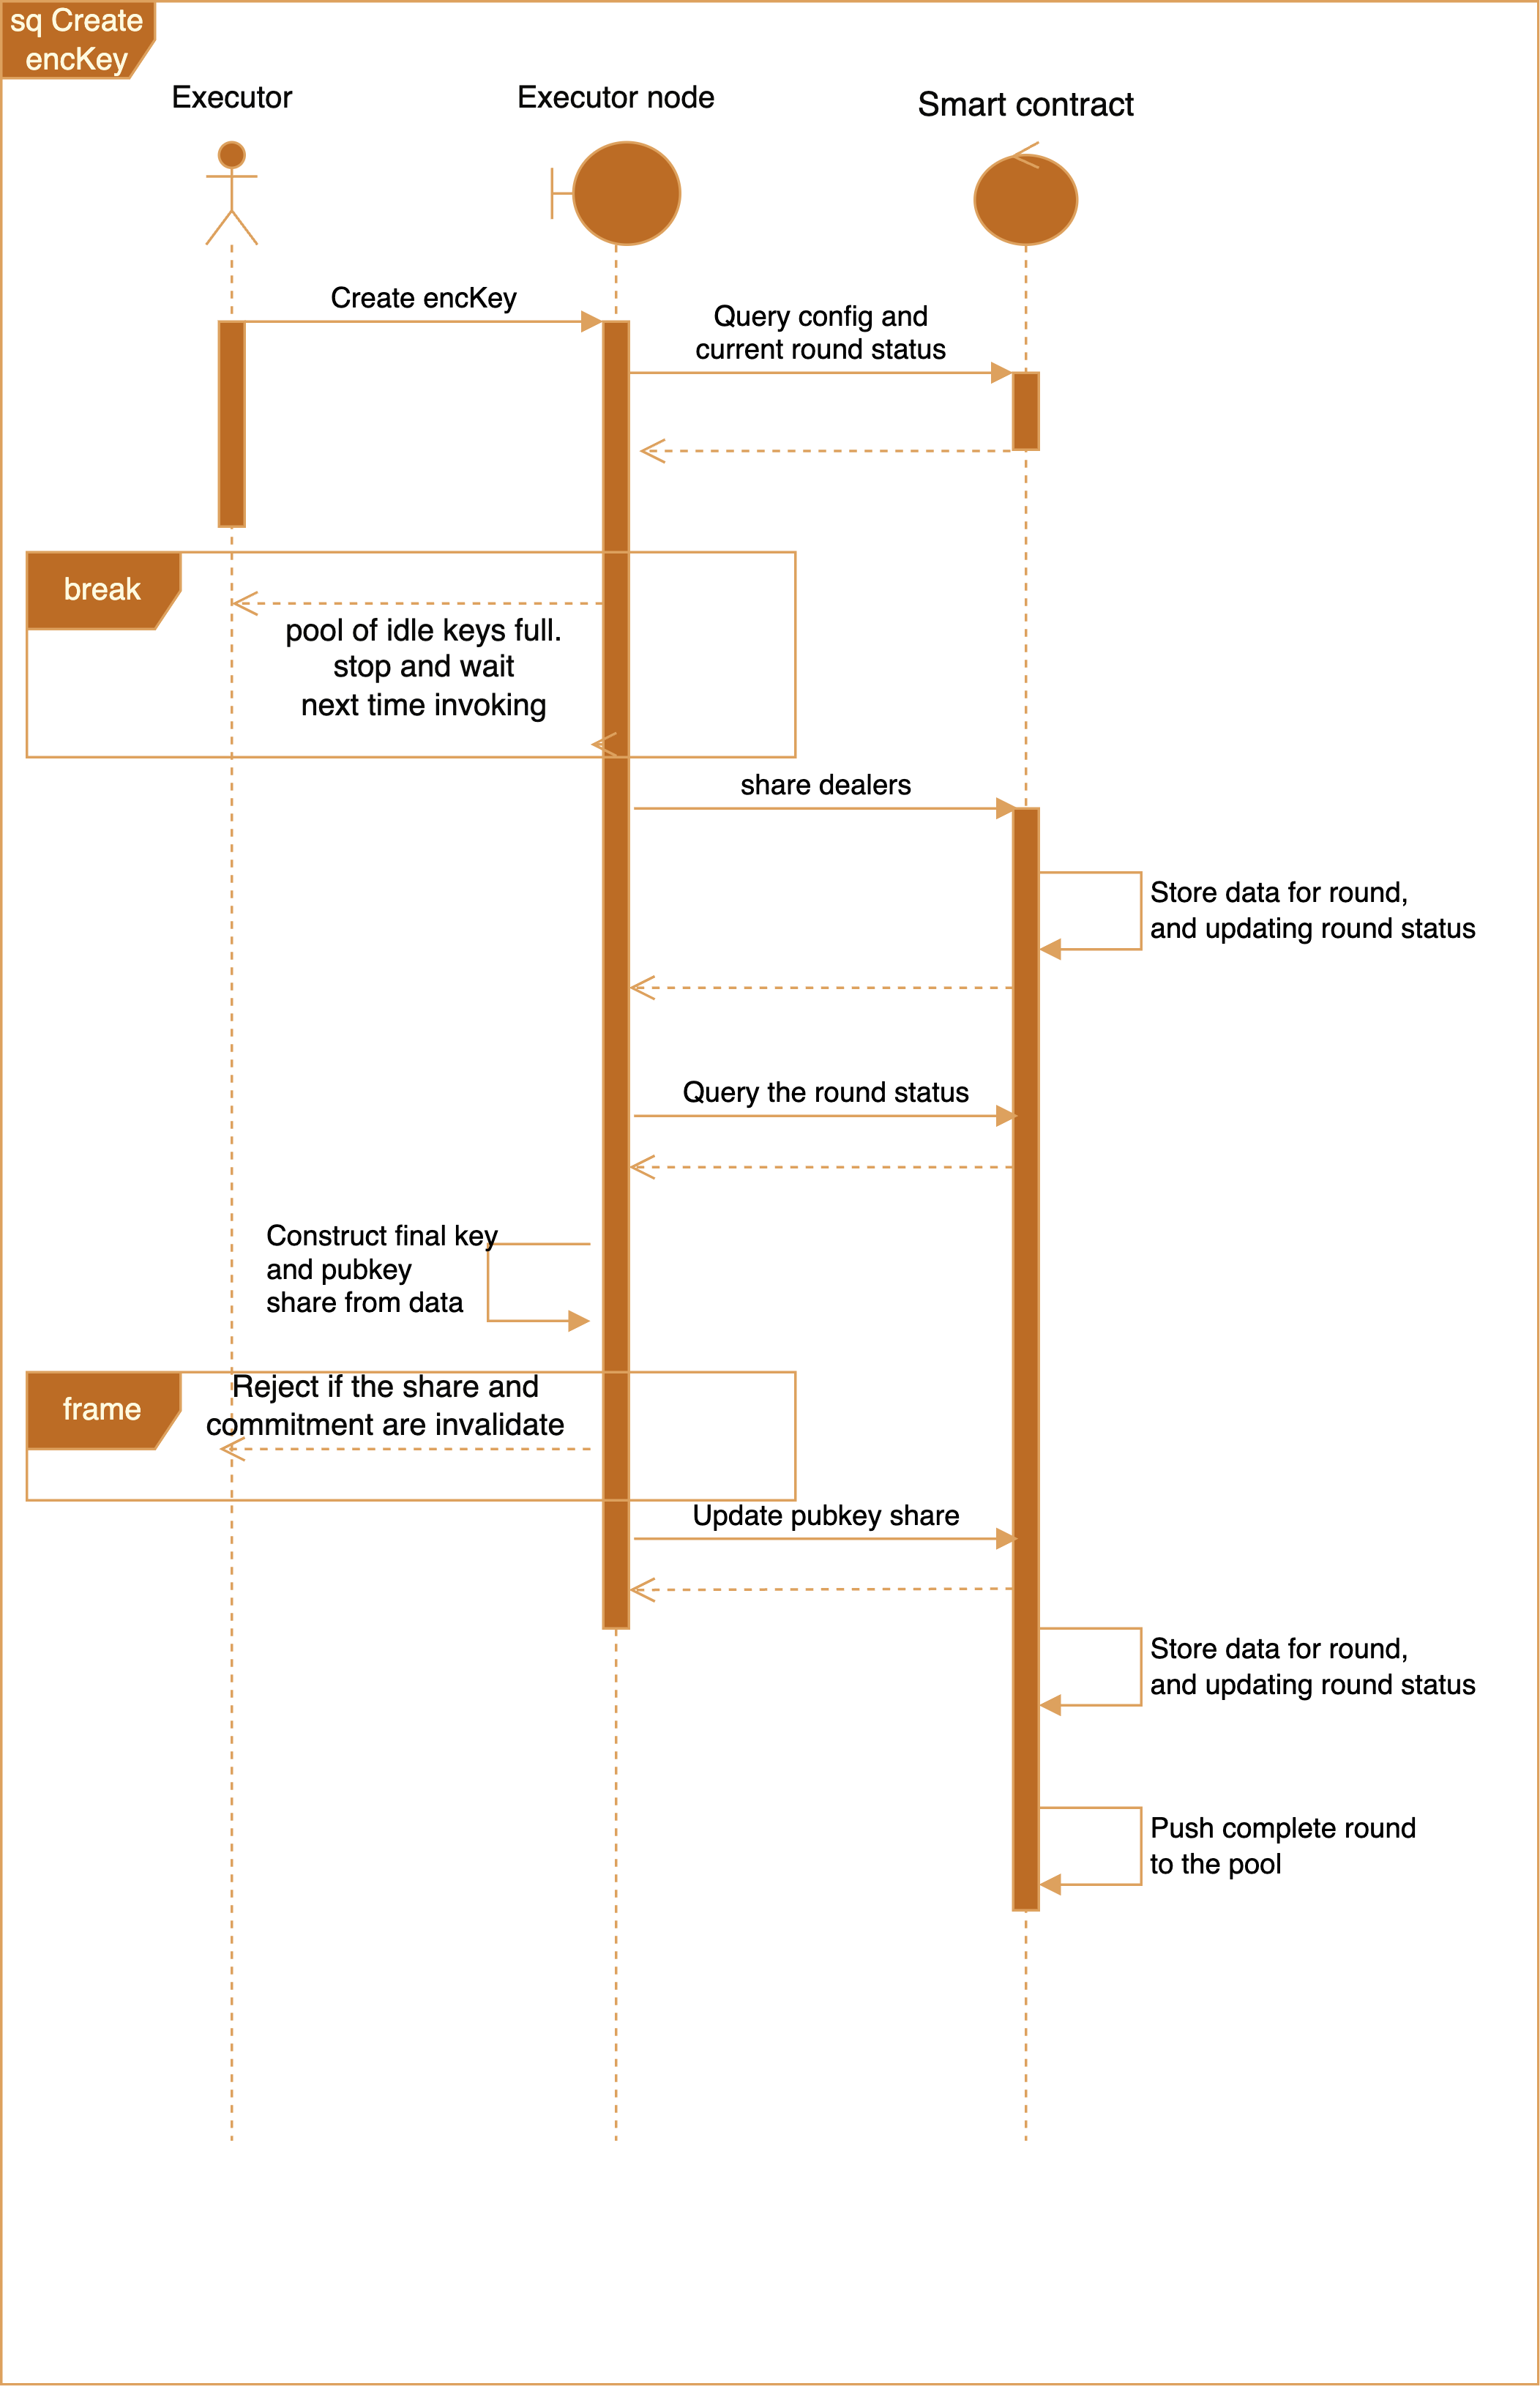
\includegraphics[scale=0.14]{Figure/create-encKey-sequence-diagram.png}
 \caption{Create encKey sequence diagram}
    \label{fig:create-encKey-sequence-diagram}
\end{figure}
Creating a new encKey in the system is a fundamental and crucial operation that has a substantial impact on the system's overall efficacy and security. This crucial procedure is initiated when the executor, acting as a specialized actor in the system, performs the required action. To optimize the role of the executor, I meticulously designed the executor node as a cron job executor, assuring seamless management and efficient task execution. By implementing the executor node as a cron job executor, I've ensured the creation of new encKeys is optimized for efficiency and seamless administration. The cron job scheduler enables the executor to perform repetitive duties automatically and at specified intervals. This ensures that the generation of new encKeys is consistent, efficient, and always ready to satisfy the system's demands.
\begin{figure}[H]
 \centering
 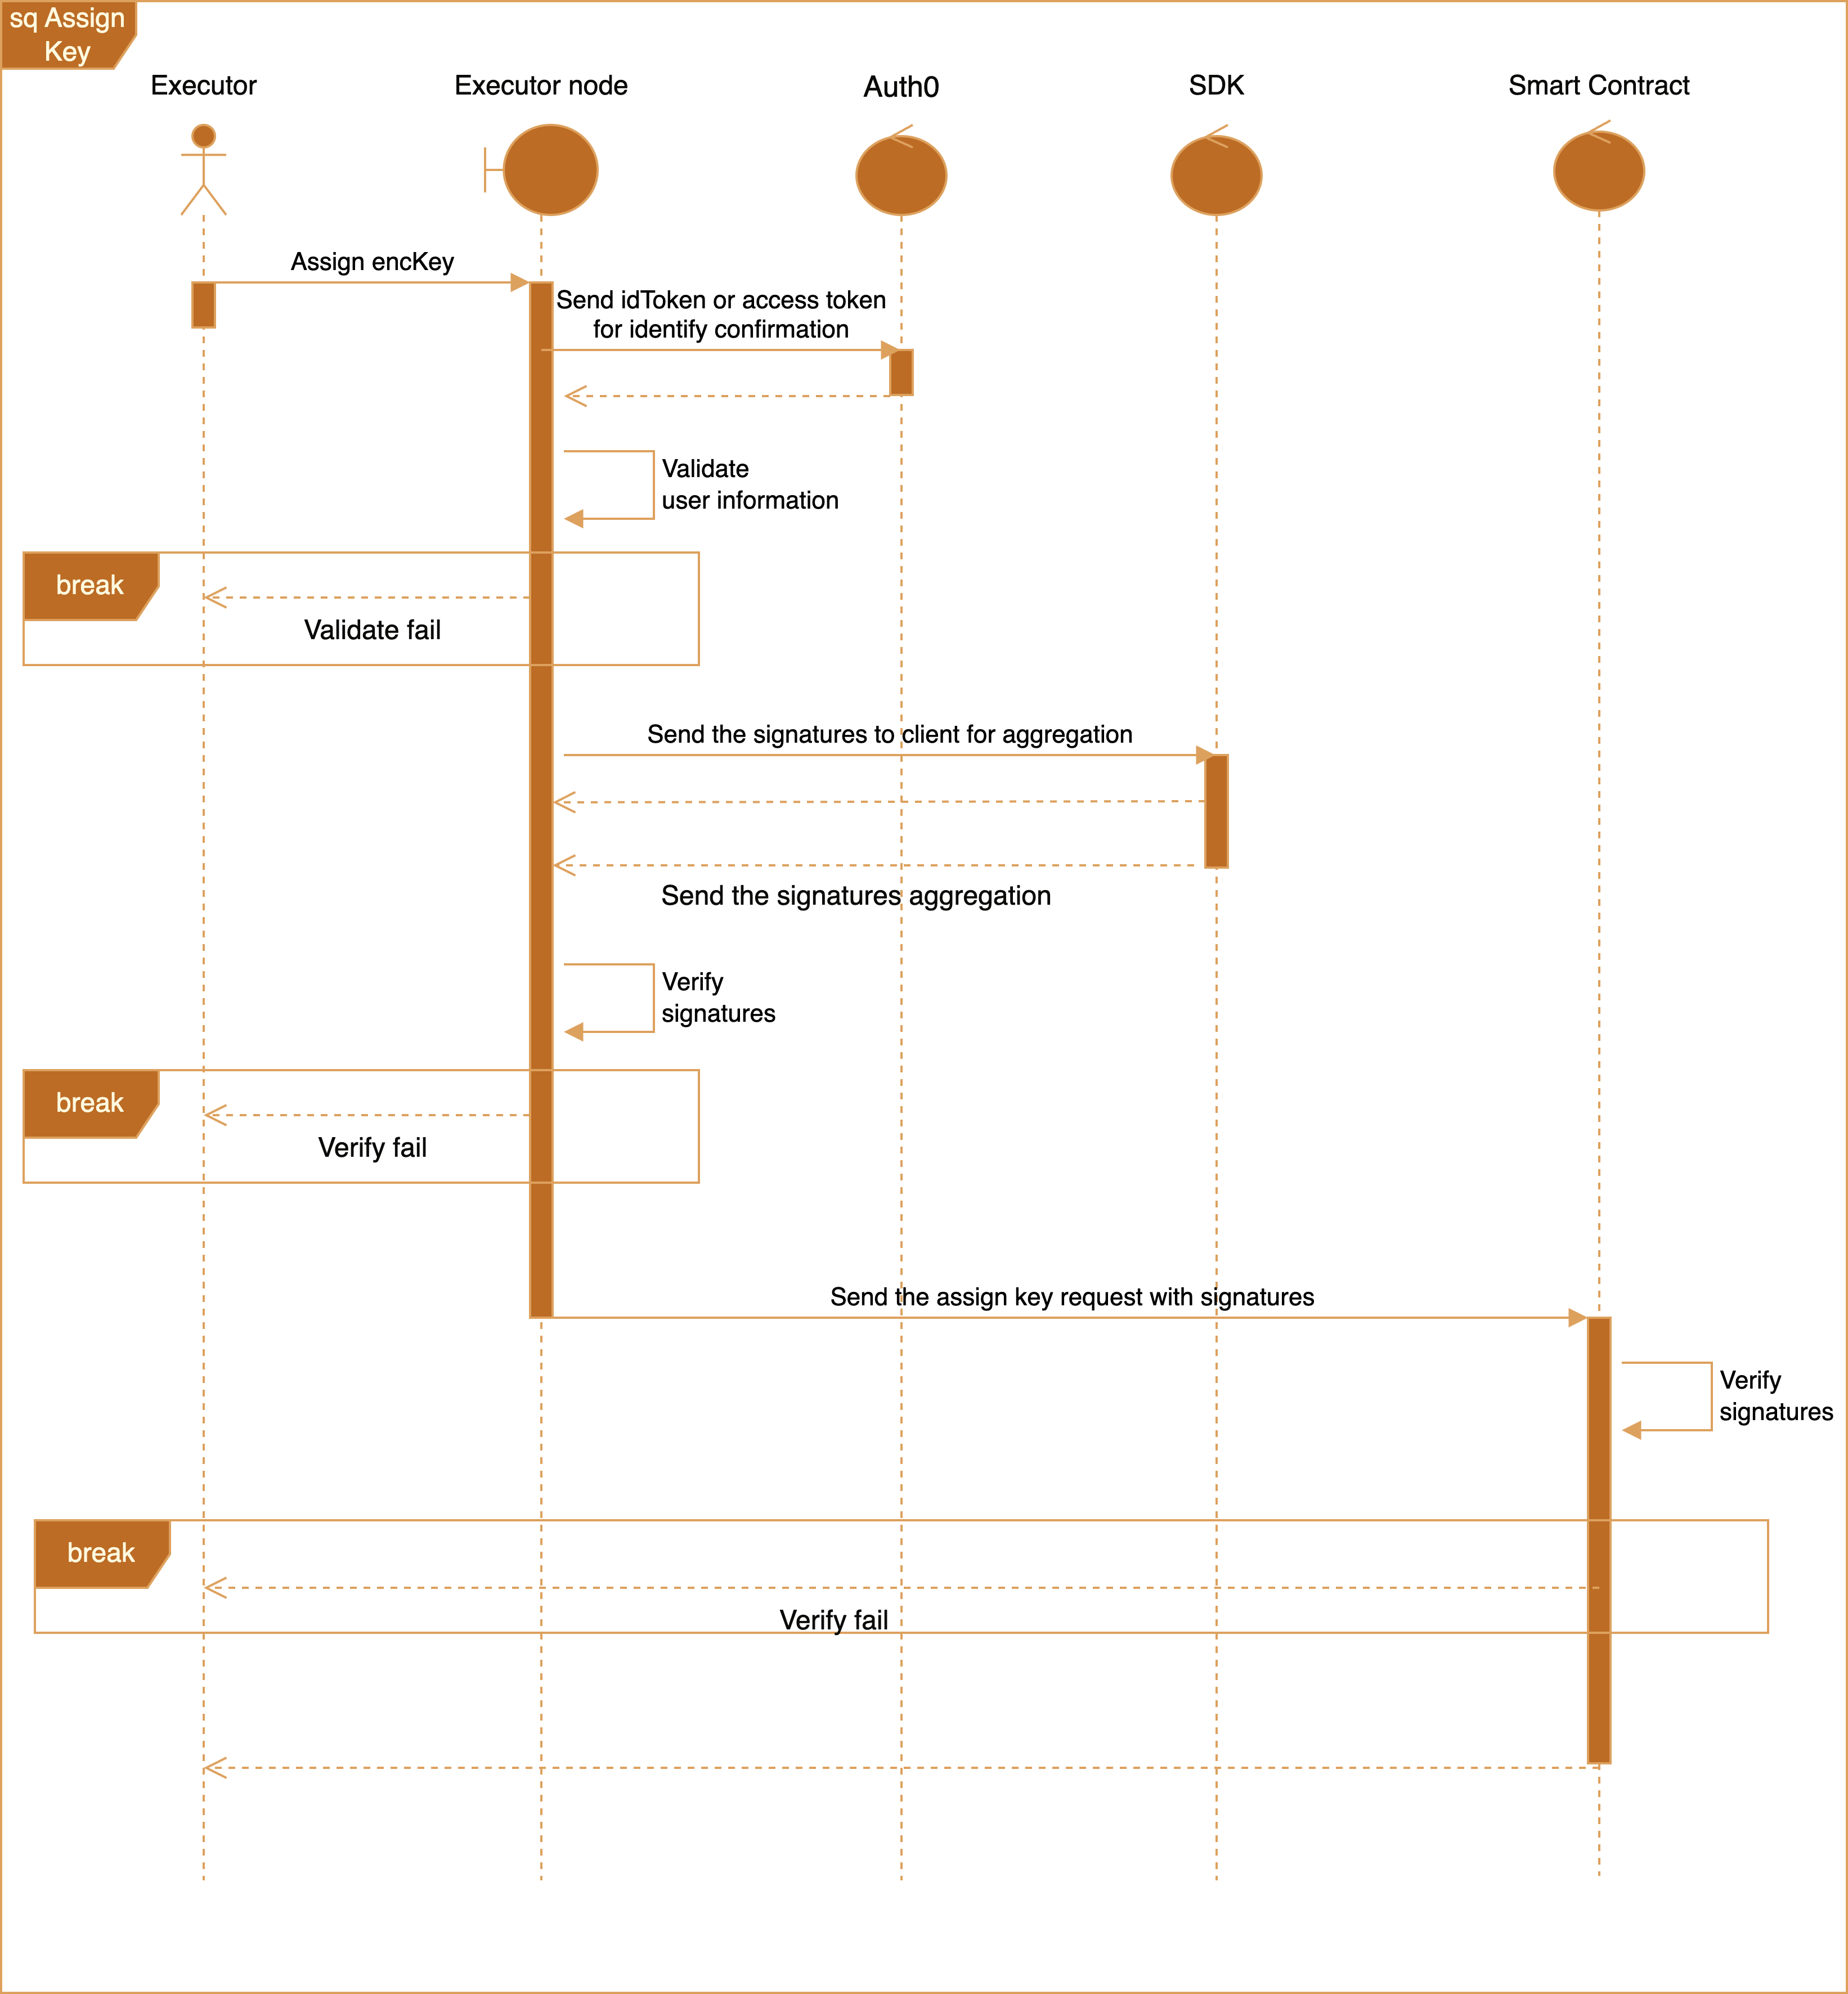
\includegraphics[scale=0.14]{Figure/assign-key-sequence-diagram.png}
 \caption{Assign encKey for user sequence diagram}
    \label{fig:assign-key-sequence-diagram}
\end{figure}
The complexity and security of the executor's procedure for allocating a new encKey to a user exemplifies the robustness of the system. When a user requests their encKey, the executor receives their data, which contains crucial validation information. Through a series of exhaustive validation tests, the executor ensures that the user's data is valid, accurate, and in accordance with the system's specifications. This validation phase is a crucial line of defense against possible data inaccuracies and unauthorized access attempts. The executor verifies the signatures of other executors who participate in the assignment procedure to increase the process's security. These signature verifications are necessary to affirm the credibility and authenticity of each executor involved in the assignment process. The system ensures that only authorized and trustworthy parties contribute to the designation of the new encKey by establishing trust among all participating executors.

\subsection{Package diagram}

\begin{figure}[H]
 \centering
 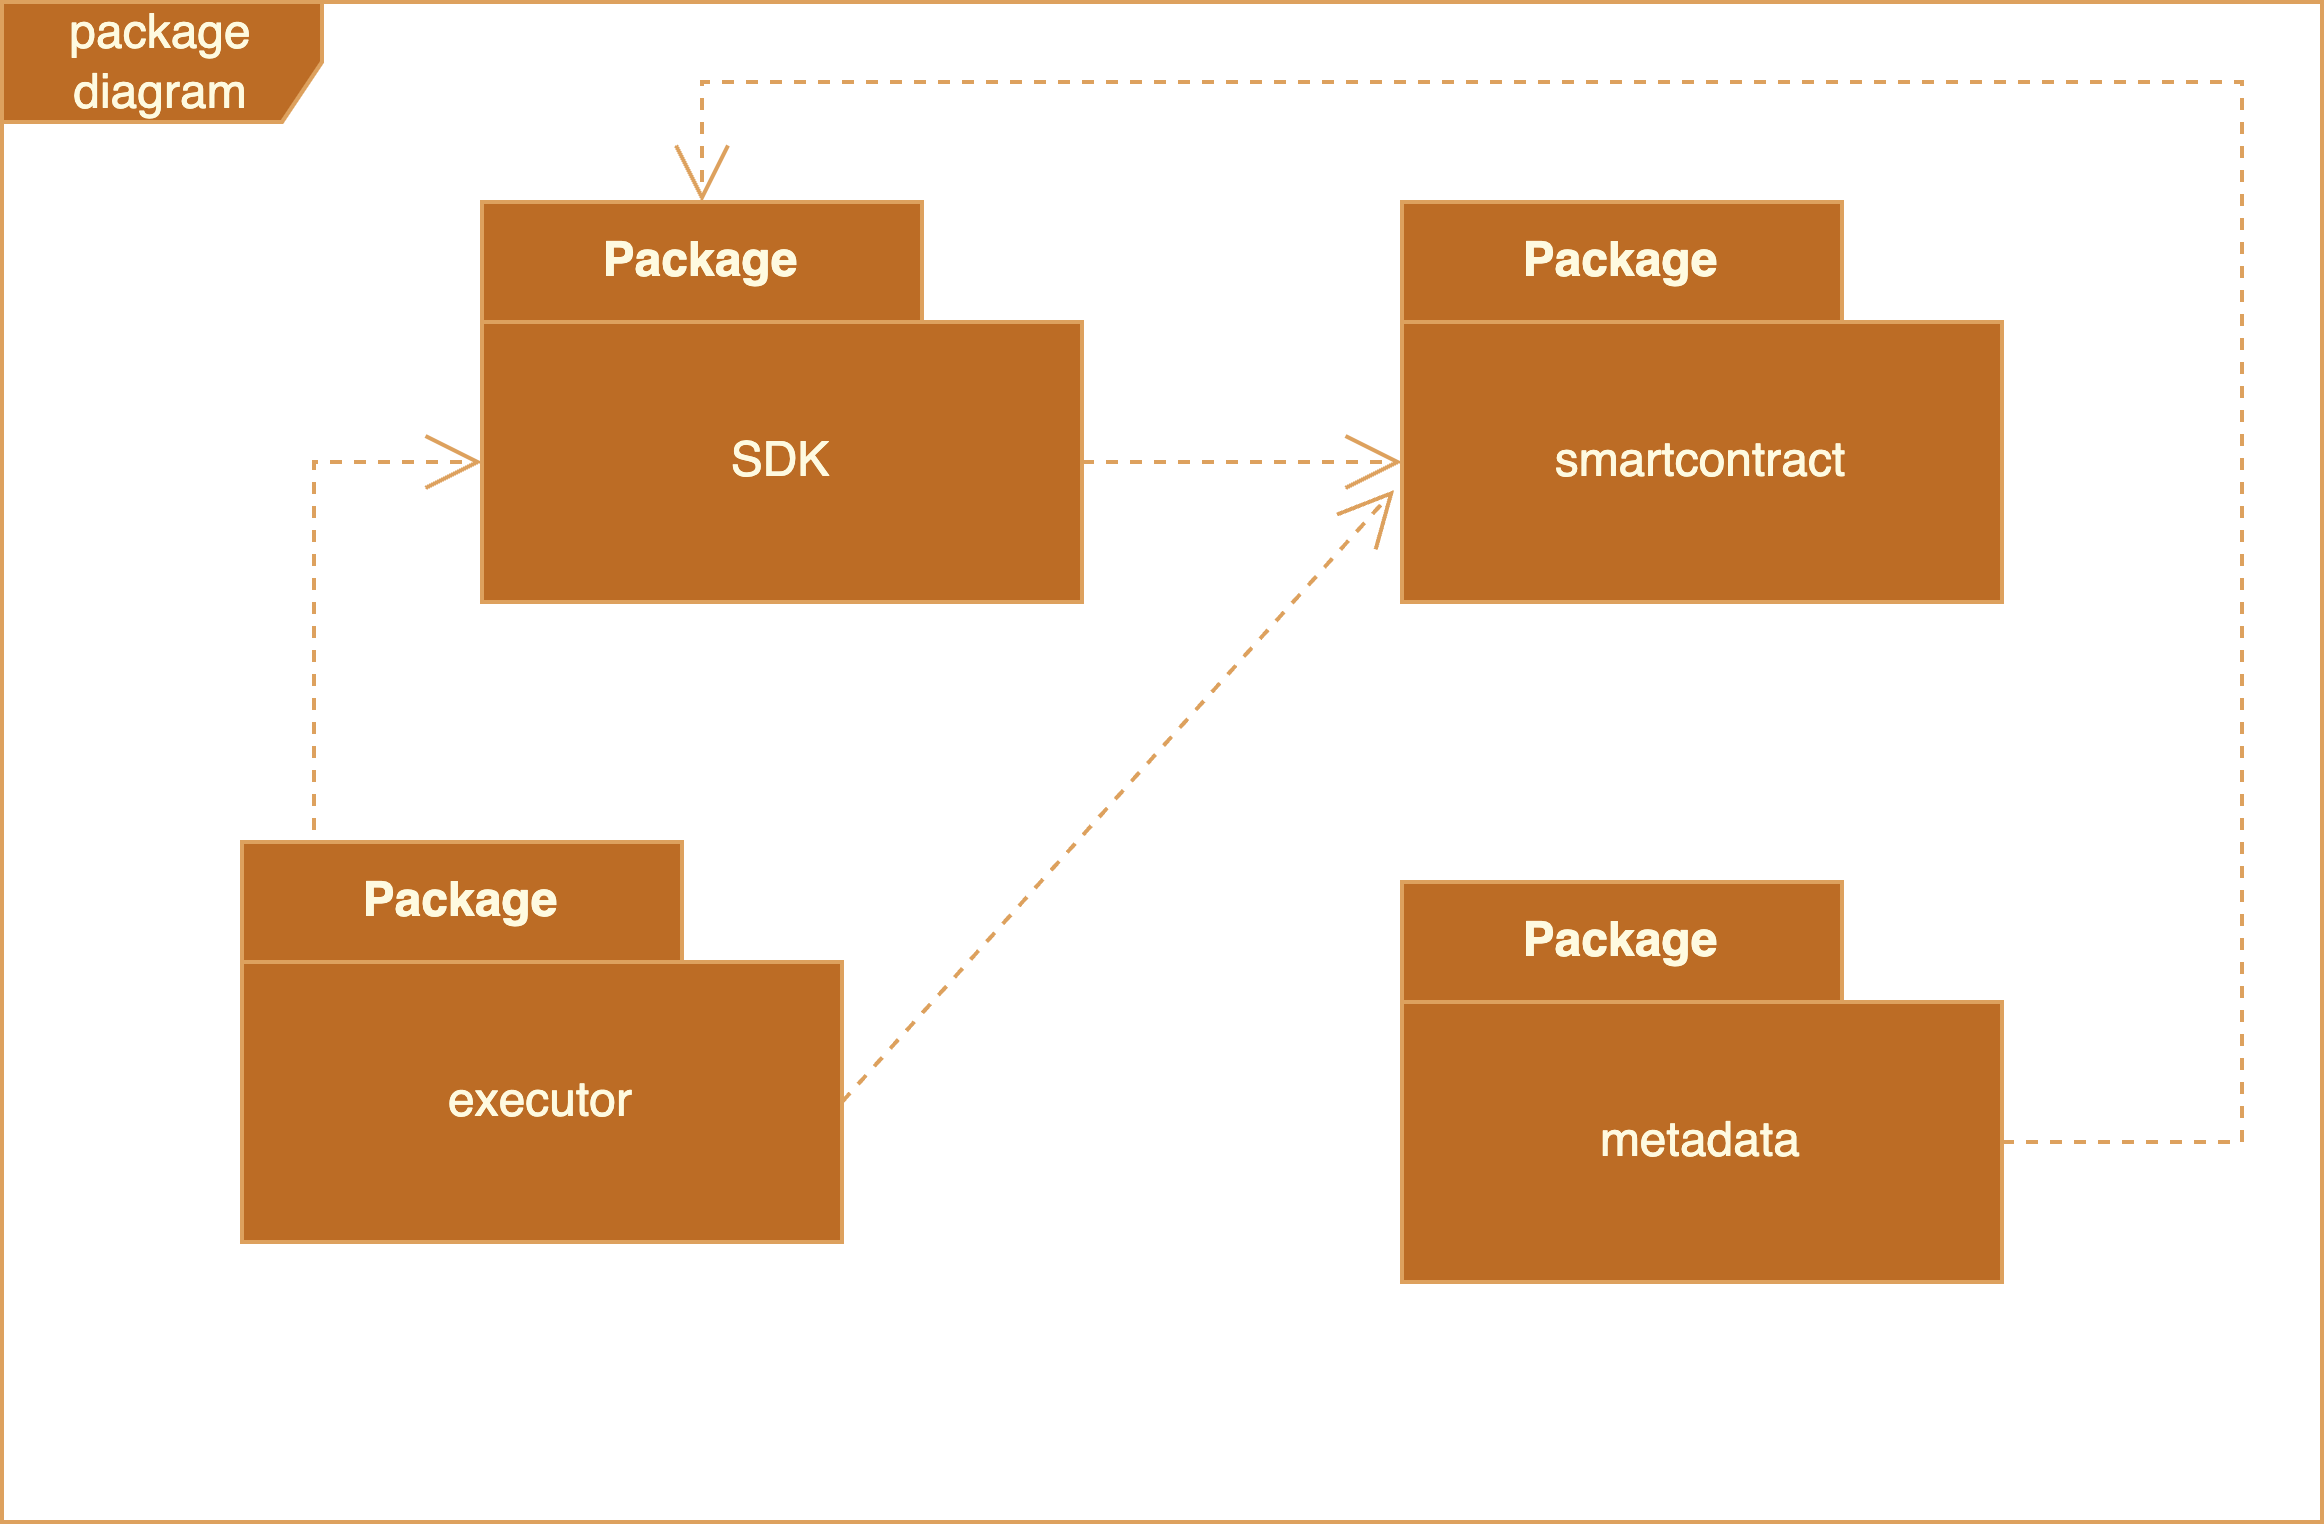
\includegraphics[scale=0.17]{Figure/package-diagram.png}
 \caption{Package diagram}
    \label{fig:package-diagram}
\end{figure}
The system's architecture has been meticulously crafted to guarantee a secure and seamless user experience within the Web3 ecosystem. Each module is essential to the overall functionality of the system, contributing to its efficacy, security, and usability. The SDK program acts as the user interface, bridging users with the system. It enables users to effortlessly interact with the system, view their private keys and shares, and execute a variety of operations. Through the SDK, users can access and administer their cryptographic keys, which are crucial for identity verification and authorization in the Web3 environment. This program provides users with an intuitive and user-friendly interface that simplifies the complexities of Web3 technologies. By encapsulating the underlying complexities, the SDK improves accessibility, allowing a wider audience to appreciate the advantages of decentralized applications and blockchain-powered services. In the meantime, the executor package serves as a vital intermediary layer that facilitates the execution of user queries. It manages client-system interactions and processes user-initiated actions on their behalf. As a fundamental system component, the executor package is responsible for generating new encKeys, the fundamental building blocks for secure user authentication and authorization. In addition, it validates user information to ensure the validity and authenticity of performed actions. By interacting with the blockchain, the executor package can implement transactions securely in accordance with the smart contract's rules and conditions. This blockchain integration provides the system with the immutability, transparency, and trustworthiness that are inherent to blockchain technology. The metadata package functions as a dependable mechanism for data storage and querying, maintaining the essential metadata associated with user identities and encKeys. This package is essential for the secure storage of user-related data in a database, ensuring data integrity and privacy. By managing SDK package queries, the metadata package retrieves and delivers query responses efficiently. It is essential for providing seamless and secure access to user data, nurturing a high level of user confidence and trust in the system. As a secure data repository, the metadata package substantially contributes to the privacy and security of the system as a whole. The interdependencies between these products are essential to the development of a cohesive and effective system. The SDK bundle is dependent on the configuration data present in the smart contract, which provides crucial information for user interactions and authentication. To execute its actions, the executor package relies on both the data stored in the smart contract and the requests from the SDK. This harmonious cooperation enables the executor to execute tasks securely while adhering to the smart contract's predefined rules and conditions. The metadata package, which stores and retrieves user-related data, complements the SDK and executor products' functionality. It assures the accessibility of vital data, facilitating data access and user interactions. By carefully orchestrating the interactions between these packages, the system accomplishes a robust and user-friendly environment. The combination of blockchain technology, social authentication, and user-controlled encryption keys ushers in a new era of secure, decentralized, and user-centric Web3 applications. The interaction between these packages constitutes the system's backbone, allowing it to leverage the benefits of Web3 while mitigating the difficulties associated with technical complexities, thereby nurturing widespread adoption and utility. The seamless integration of these products empowers users, streamlines their Web3 experience, and instills confidence in the system's security and dependability.

\subsection{Entity diagram}
In the context of the centralized system described in this thesis, it is possible that the traditional Entity-Relationship (ER) diagram does not completely capture the unique characteristics of the metadata storage in the smart contract. Instead, we can depict the entities and their relationships within the system using an alternate representation. This system's smart contract serves as the central repository for metadata associated with user identities and encKeys. It operates as a decentralized database, storing and managing user-specific data on the blockchain using key-value pairings. The key-value approach is ideally suited for the metadata module because it facilitates efficient data retrieval and assures data integrity and immutability. In this context, the entities and their relationships can be described as follows:
\begin{figure}[H]
 \centering
 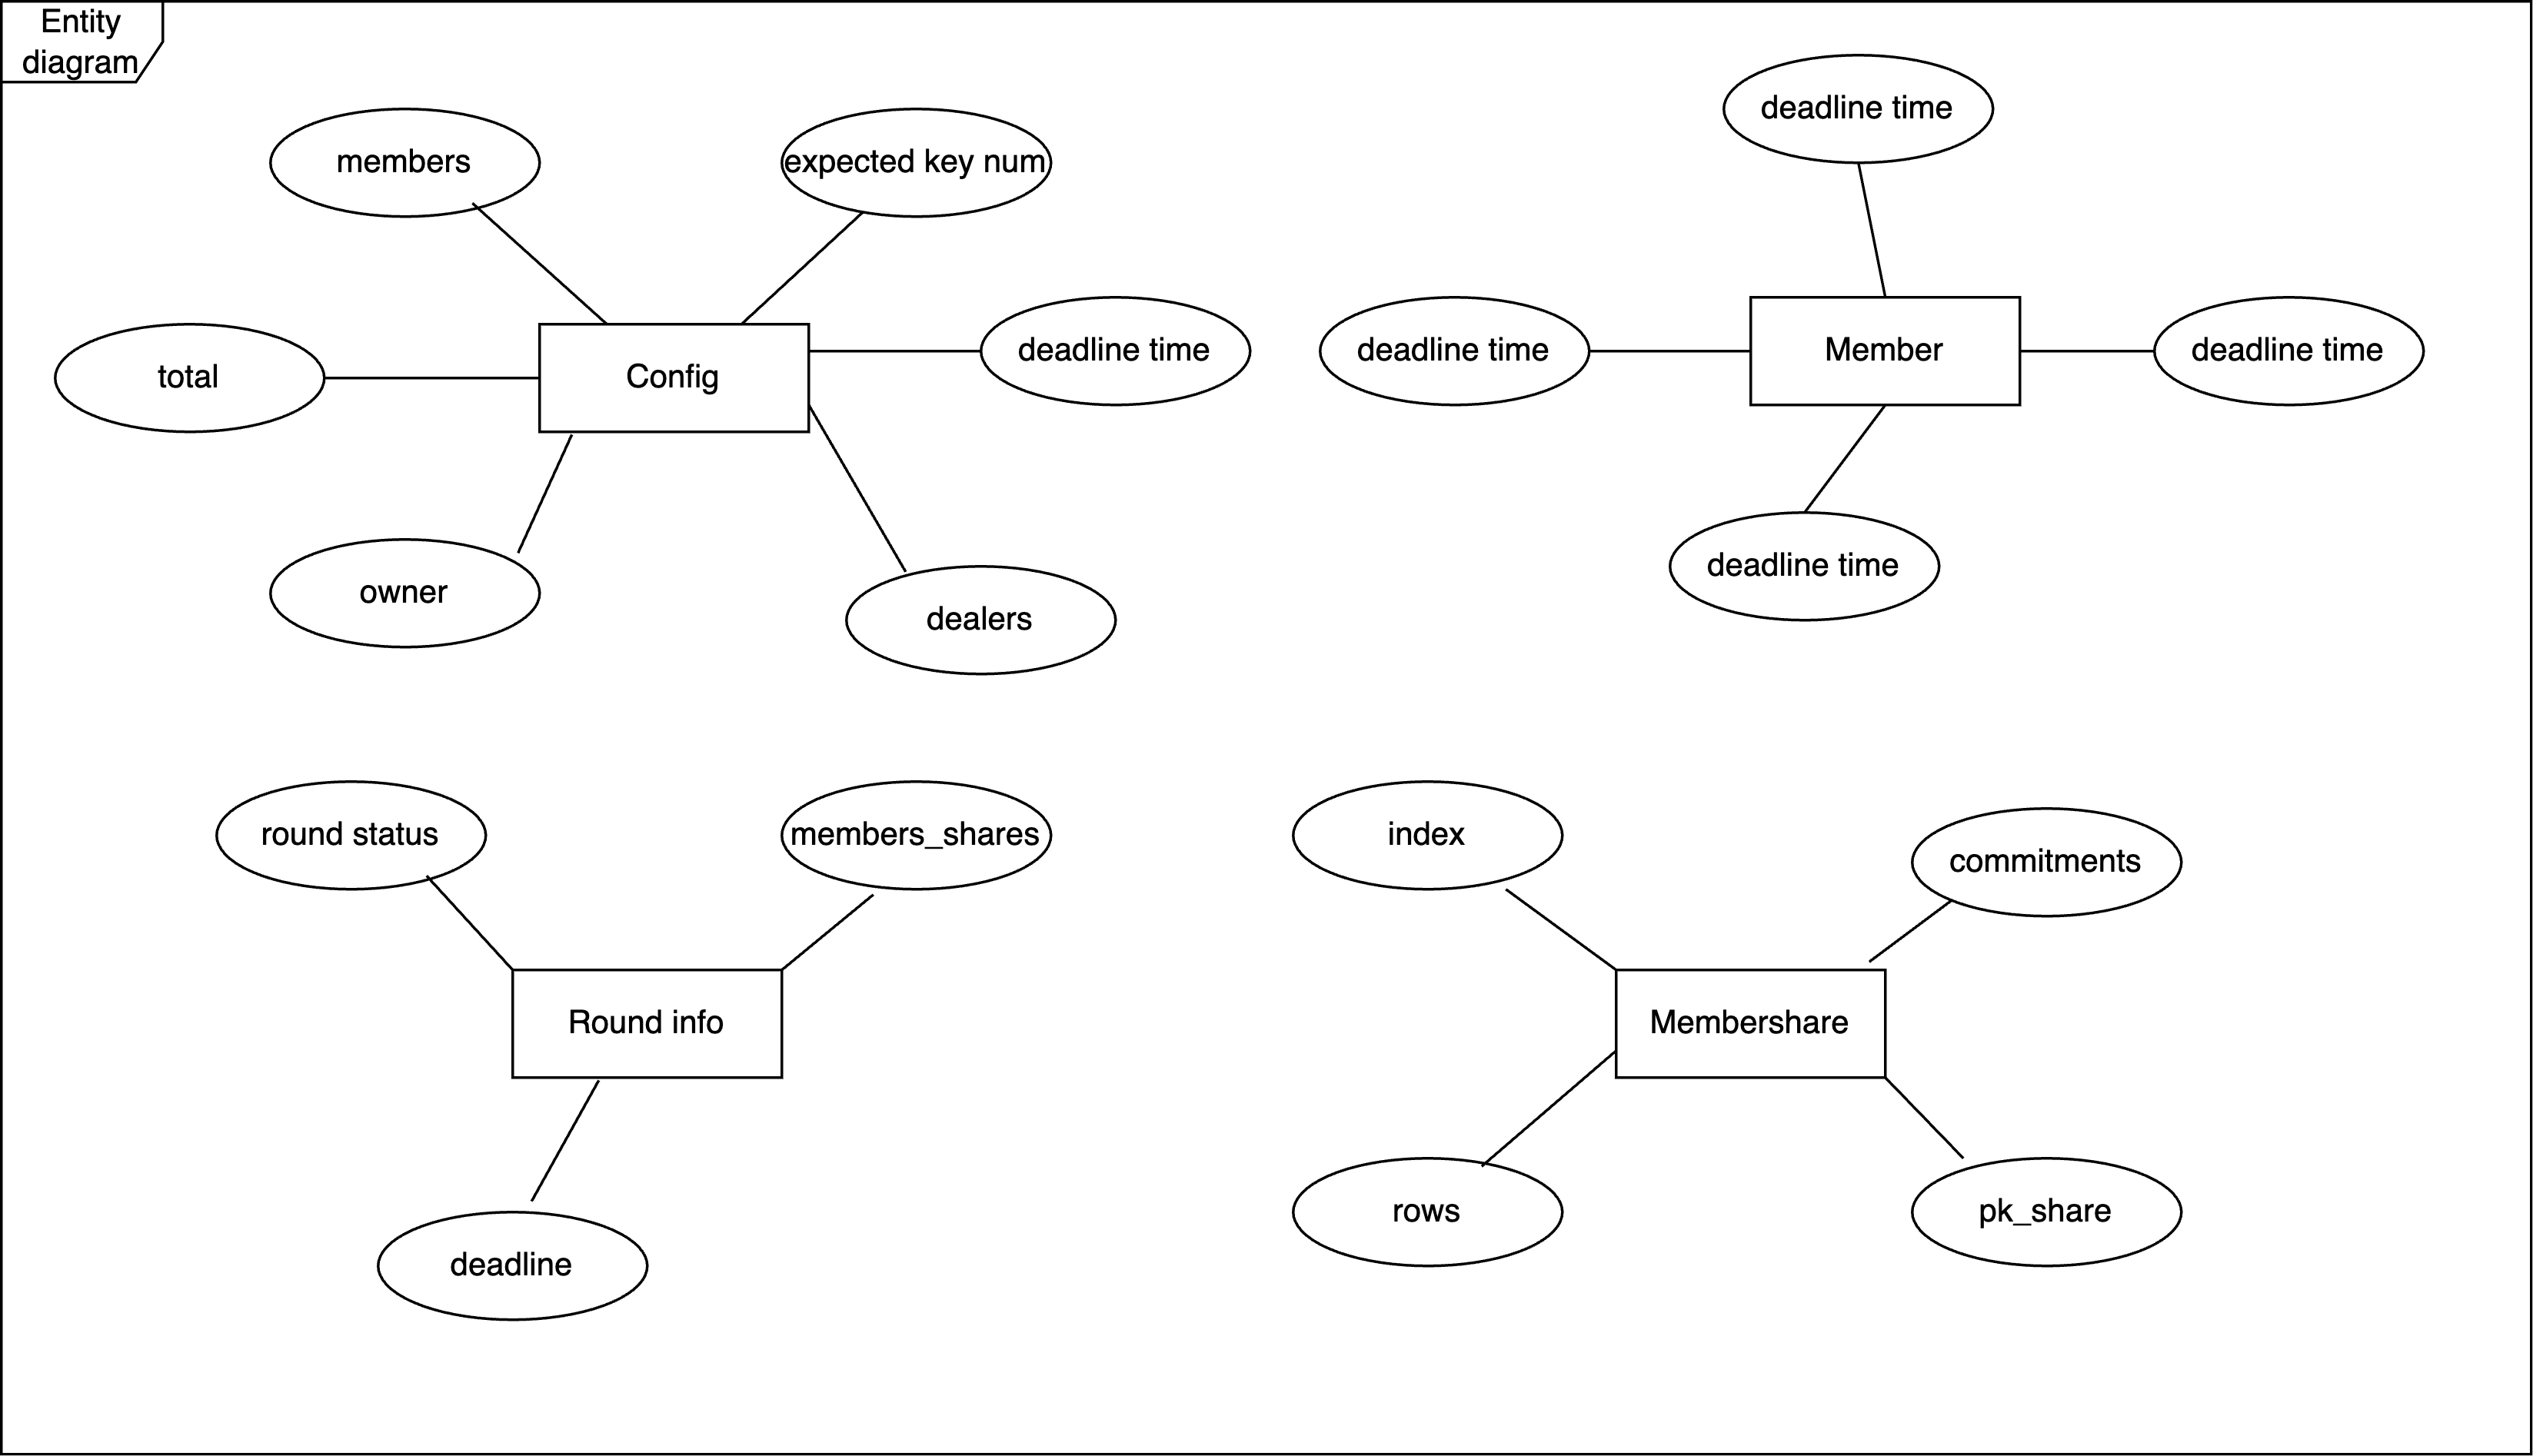
\includegraphics[scale=0.13]{Figure/entity-diagram.png}
 \caption{Entity diagram}
    \label{fig:entity-diagram}
\end{figure}
All the strong entities that are stored directly as states are underlined with unique keys in the diagram. Since states are stored using key-value pairings, similar to a document-oriented database, it is unnecessary to have relationships between the entities.\\

The entity particulars are detailed in the tables that follow:
\begin{table}[H]
  \centering
  \begin{tabular}{|l|l|l|p{9cm}|}
\hline
\rowcolor[HTML]{F56B00} 
\textbf{Attribute}               & \textbf{Type} & \textbf{Required} & \textbf{Description}                                                                \\ \hline
\cellcolor[HTML]{FFFFFF}index    & number        & yes               & The index of the member in the system plays vital role in reconstructing the encKey \\ \hline
\cellcolor[HTML]{FFFFFF}pub\_key & Binary        & yes               & The pubkey of the executor participating in the system                              \\ \hline
\cellcolor[HTML]{FFFFFF}address  & Addr          & yes               & The address of the executor participating in the system                             \\ \hline
end\_point                       & string        & yes               & end\_point is the url to executor node, which for the request in the SDK            \\ \hline
\end{tabular}
 \caption{Member entity detail}
    \label{fig:member-entity-detail}
\end{table}

\begin{table}[H]
    \centering
    \begin{tabular}{|l|l|l|p{7cm}|}
\hline
\rowcolor[HTML]{F56B00} 
\textbf{Attribute}              & \textbf{Type}                      & \textbf{Required} & \textbf{Description}                                              \\ \hline
\cellcolor[HTML]{FFFFFF}members & Vec\textless{}Member\textgreater{} & yes               & The member or executors operate the system                        \\ \hline
\cellcolor[HTML]{FFFFFF}total   & number                             & yes               & Total member participate in the system                            \\ \hline
\cellcolor[HTML]{FFFFFF}owner   & Addr                               & yes               & The address of the owner of the system                            \\ \hline
expected\_key\_num              & number                             & yes               & The number of expected keys are in idle pool                      \\ \hline
deadline\_time                  & number                             & yes               & The maxium duration of creating a key                             \\ \hline
dealers                         & number                             & yes               & Thresholds for the 2 phase "Wait for dealers" and "Wait for rows" \\ \hline
\end{tabular}
 \caption{Config entity detail}
    \label{fig:config-entity-detail}
\end{table}

\begin{table}[H]
  \centering
  \begin{tabular}{|l|l|l|p{8cm}|}
\hline
\rowcolor[HTML]{F56B00} 
\textbf{Attribute}                  & \textbf{Type}                      & \textbf{Required} & \textbf{Description}                               \\ \hline
\cellcolor[HTML]{FFFFFF}index       & number                             & yes               & The index of executor in the system                \\ \hline
\cellcolor[HTML]{FFFFFF}commitments & Vec\textless{}Binary\textgreater{} & no                & The commitments of shares of executor for the rows \\ \hline
\cellcolor[HTML]{FFFFFF}rows        & Vec\textless{}Binary\textgreater{} & no                & The encrypted shares for other executors           \\ \hline
pk\_share                           & Binary                             & no                & The pubkey of the final share of executor          \\ \hline
\end{tabular}
 \caption{Membershare entity detail}
    \label{fig:membershare-entity-detail}
\end{table}

\begin{table}[H]
  \centering
  \begin{tabular}{|l|l|l|p{7cm}|}
\hline
\rowcolor[HTML]{F56B00} 
\textbf{Attribute}                     & \textbf{Type}                           & \textbf{Required} & \textbf{Description}                                                                                             \\ \hline
\cellcolor[HTML]{FFFFFF}round\_status  & number                                  & yes               & The status of the round, there are 4 status include in: WaitForDealers, WaitForRows, WaitForAssign, and Assigned \\ \hline
\cellcolor[HTML]{FFFFFF}member\_shares & Vec\textless{}Membershare\textgreater{} & no                & The shares of executor for round                                                                                 \\ \hline
\cellcolor[HTML]{FFFFFF}deadline       & Vec\textless{}Binary\textgreater{}      & no                & The deadline of this round                                                                                       \\ \hline
\end{tabular}
 \caption{RoundInfo entity detail}
    \label{fig:roundinfo-entity-detail}
\end{table}

\section{Message design}
\subsection{Smart contract message}
CosmWasm \cite{cosmwasm} is a smart contract platform that has been developed utilizing the Cosmos SDK\cite{cosmos-sdk}, a blockchain framework specifically designed for the construction of DApps. CosmWasm offers a robust and optimized framework for the execution of intelligent contracts across diverse blockchain networks, ensuring both security and efficiency. The CosmWasm smart contract model is founded upon the actor model, a widely adopted paradigm utilized in the design of concurrent and distributed systems. The actor model is a computational paradigm in which each smart contract is conceptualized as an actor. An actor is an autonomous entity capable of receiving messages, performing computations on them, and transmitting messages to other actors. In the CosmWasm smart contract model, the actors are characterized by their isolation from one another, with communication occurring exclusively through the exchange of messages.
\subsubsection{Instantiate message}
The concept of instantiation messages pertains to the process of instantiating and deploying a smart contract on the blockchain.
\begin{table}[H]
  \centering
  \begin{tabular}{|l|l|l|p{8cm}|}
\hline
\rowcolor[HTML]{F56B00} 
\textbf{Field}                  & \textbf{Type}                      & \textbf{Required} & \textbf{Description}                                   \\ \hline
\cellcolor[HTML]{FFFFFF}members  & Vec\textless{}Member\textgreater{} & yes               & The information of executors participate in the system \\ \hline
\cellcolor[HTML]{FFFFFF}dealers & u8                                 & yes               & Thresholds of the system for passing each phase        \\ \hline
owner                           & string                             & yes               & Owner of the smart contract                            \\ \hline
expected\_key\_num              & uint                               & yes               & The expected number of key in idle pool                \\ \hline
deadline\_time                  & uint                               & yes               & The maxium duration of 1 round                         \\ \hline
\end{tabular}
  \caption{Instantiate message detail}
  \label{instantiate-message-detail}
\end{table}
\subsubsection{Execute message}
The execute message serves as the primary interface for processing incoming messages and executing the contract's logic in accordance with the provided input. Every execute message contained within the executor message enumeration possesses a distinct structure and data payload, thereby empowering the smart contract to effectively react to a wide array of interactions originating from users or other entities within the blockchain ecosystem.\\

The following tables provide a more comprehensive description of each execute message:\\
\begin{table}[H]
  \centering
  \begin{tabular}{|l|l|l|p{8cm}|}
\hline
\rowcolor[HTML]{F56B00} 
\textbf{Field}                      & \textbf{Type}                      & \textbf{Required} & \textbf{Description}                                                                                         \\ \hline
\cellcolor[HTML]{FFFFFF}rows        & Vec\textless{}Binary\textgreater{} & yes               & The shares given to each participant in the DKG protocol in order to construct their final share for encKey. \\ \hline
\cellcolor[HTML]{FFFFFF}commitments & Vec\textless{}Binary\textgreater{} & yes               & The commitments are to confirm that the rows originate from the precise source                               \\ \hline
\end{tabular}
  \caption{ShareDealerMsg detail}
  \label{sharedealer-msg-detail}
\end{table}

\begin{table}[H]
  \centering
  \begin{tabular}{|l|l|l|p{8cm}|}
\hline
\rowcolor[HTML]{F56B00} 
\textbf{Field}                    & \textbf{Type} & \textbf{Required} & \textbf{Description}                                                                                                        \\ \hline
\cellcolor[HTML]{FFFFFF}pk\_share & Binary        & yes               & pk\_share is the pubkey of the final share that the executor reconstructs using rows and commitments from the share dealer. \\ \hline
\end{tabular}
  \caption{ShareRowMsg detail}
  \label{sharerow-msg-detail}
\end{table}

\begin{table}[H]
  \centering
  \begin{tabular}{|l|l|l|p{8cm}|}
\hline
\rowcolor[HTML]{F56B00} 
\textbf{Field}                  & \textbf{Type} & \textbf{Required} & \textbf{Description}                        \\ \hline
\cellcolor[HTML]{FFFFFF}members & MemberMsg     & no                & The member config                           \\ \hline
owner                           & string        & no                & The new owner                               \\ \hline
dealers                         & u8            & no                & The new thresholds                          \\ \hline
expected\_key\_num              & uint          & no                & The new expected number of key in idle pool \\ \hline
deadline\_time                  & uint          & no                & The new maxium duration of key creation     \\ \hline
\end{tabular}
  \caption{UpdateConfigMsg detail}
  \label{updateconfig-msg-detail}
\end{table}

\begin{table}[H]
  \centering
  \begin{tabular}{|l|l|l|p{8cm}|}
\hline
\rowcolor[HTML]{F56B00} 
\textbf{Field}               & \textbf{Type}                      & \textbf{Required} & \textbf{Description}                                                    \\ \hline
\cellcolor[HTML]{FFFFFF}sigs & Vec\textless{}Binary\textgreater{} & yes               & The signatures of the executor which approve for assigning key for user \\ \hline
pub\_key                     & Vec\textless{}Binary\textgreater{} & yes               & The pubkey of the executors that create the signature                   \\ \hline
verifier                     & string                             & yes               & The name of app which is whitelisted in the system                      \\ \hline
verifier\_id                 & string                             & yes               & email or user\_id                                                       \\ \hline
\end{tabular}
  \caption{AssignKeyMsg detail}
  \label{assignkey-msg-detail}
\end{table}

\begin{table}[H]
  \centering
  \begin{tabular}{|l|l|l|p{8cm}|}
\hline
\rowcolor[HTML]{F56B00}
\textbf{Field} & \textbf{Type} & \textbf{Required} & \textbf{Description}                               \\ \hline
verifier       & string        & yes               & The name of app which is whitelisted in the system \\ \hline
client\_id     & string        & yes               & The client\_id of the app                          \\ \hline
\end{tabular}
  \caption{UpdateVerifierMsg detail}
  \label{updateverifier-msg-detail}
\end{table}

\subsubsection{Query message}
QueryMsg is a specific variety of execute message within the executor message enum within the context of the CosmWasm smart contract and actor model. It is designed to manage query requests and enables the smart contract to provide read-only, non-modifiable access to its current state. When a query request is received, the smart contract processes the QueryMsg and executes the required operations to retrieve the requested information from its internal state. As a response to the inquiry, the smart contract can then construct and return the requested data. \\
\indent The query messages and responses schema are desbribed in detail by the following tables:\\
\begin{table}[H]
  \centering
  \begin{tabular}{|l|l|l|p{8cm}|}
\hline
\rowcolor[HTML]{F56B00}
\textbf{Field}  & \textbf{Type}                           & \textbf{Required} & \textbf{Description}                            \\ \hline
round\_id       & uint                                    & yes               & The id of the round                             \\ \hline
round\_status   & usize                                   & yes               & The status of the round                         \\ \hline
members\_shares & Vec\textless{}MemberShare\textgreater{} & yes               & The details about the membershares of the round \\ \hline
deadline        & uint                                    & yes               & The deadline of the round                       \\ \hline
\end{tabular}
  \caption{RoundInfoResponse detail}
  \label{roundinfo-response-detail}
\end{table}

\begin{table}[H]
  \centering
  \begin{tabular}{|l|l|l|p{8cm}|}
\hline
\rowcolor[HTML]{F56B00}
\textbf{Field}     & \textbf{Type}                      & \textbf{Required} & \textbf{Description}                                        \\ \hline
members            & Vec\textless{}Member\textgreater{} & yes               & The information of the executor participating in the system \\ \hline
total              & uint                               & yes               & The number of the executor                                  \\ \hline
dealer             & uint                               & yes               & Thresholds of the system                                    \\ \hline
owner              & string                             & yes               & Owner of the system                                         \\ \hline
expected\_key\_num & uint                               & yes               & The number of expected keys in idle pool                    \\ \hline
\end{tabular}
  \caption{ConfigResponse detail}
  \label{config-response-detail}
\end{table}

\begin{table}[H]
  \centering
  \begin{tabular}{|l|l|l|p{8cm}|}
\hline
\rowcolor[HTML]{F56B00} 
\textbf{Field} & \textbf{Type} & \textbf{Required} & \textbf{Description}                  \\ \hline
verifier       & string       & yes               & The app that need to query user email \\ \hline
start\_after   & string        & yes               & The exclude bound start of the query  \\ \hline
limit          & uint          & no                & Number of verifierId. Default is 10   \\ \hline
\end{tabular}
  \caption{ListVerifierIdMsg detail}
  \label{listverifierid-msg-detail}
\end{table}

\begin{table}[H]
  \centering
  \begin{tabular}{|l|l|l|p{8cm}|}
\hline
\rowcolor[HTML]{F56B00} 
\textbf{Field}     & \textbf{Type}                      & \textbf{Required} & \textbf{Description}                     \\ \hline
verifier           & string                             & yes               & The app that need to query user email    \\ \hline
list\_verifier\_id & Vec\textless{}string\textgreater{} & yes               & List of the email or user\_id of the app \\ \hline
\end{tabular}
  \caption{ListVerifierIdResponse detail}
  \label{listverifierid-response-detail}
\end{table}

\begin{table}[H]
  \centering
  \begin{tabular}{|l|l|l|p{8cm}|}
\hline
\rowcolor[HTML]{F56B00} 
\textbf{Field} & \textbf{Type}                      & \textbf{Required} & \textbf{Description}                           \\ \hline
msg            & Binary                             & yes               & The mesage that was signed by executor         \\ \hline
sigs           & Vec\textless{}Binary\textgreater{} & yes               & Signatures for the message                     \\ \hline
pub\_keys      & Vec\textless{}Binary\textgreater{} & yes               & The public key of executors signed the message \\ \hline
\end{tabular}
  \caption{VerifyMemberMsg detail}
  \label{verifymember-msg-detail}
\end{table}

\subsection{JRPC message}
The executor plays a crucial role in the creation and distribution of encryption keys to users. The executor exposes four essential JSON-RPC (JRPC) methods to facilitate this functionality:\\
\indent \textbf{AssignKeyCommitmentRequest} - The executor uses this JRPC method to request the user's commitment to a new encryption key. The user will commit to the key without disclosing its actual value. This phase verifies that the user intends to generate a valid encryption key.\\
\indent \textbf{AssignKeyRequest} - The executor uses this JRPC method to request the actual encryption key from the user after obtaining the user's commitment. The user will provide the encrypted key in accordance with the commitment, ensuring that the key remains secret until later phases of the process.\\
\indent \textbf{CommitmentRequest} - The executor uses this JRPC method to request the commitments made by other executors in the system. To proceed with the encryption key generation process and accomplish the desired level of security and consensus, other executors' commitments are required.\\
\indent \textbf{ShareRequest} - Lastly, the executor uses the ShareRequest JRPC method to request shares from other executors in order to reconstruct the encryption key. As part of the distributed key generation protocol, the executor must obtain portions from multiple other executors.\\

The subsequent tables illustrate in depth the specifics of message and response:\\

\begin{table}[H]
  \centering
  \begin{tabular}{|l|l|l|p{8cm}|}
\hline
\rowcolor[HTML]{F56B00} 
\textbf{Field} & \textbf{Type} & \textbf{Required} & \textbf{Description}                                                                              \\ \hline
jsonrpc        & string        & yes               & The version of JRPC. Must be "2.0"                                                                \\ \hline
method         & string        & yes               & The method will call in the json-rpc server                                                       \\ \hline
id             & number        & yes               & An identifier established by the Client                                                           \\ \hline
params         & Object        & yes               & A Structured value that holds the parameter values to be used during the invocation of the method \\ \hline
\end{tabular}
  \caption{General JPRC request detail}
  \label{generaljrpc-request-detail}
\end{table}

\begin{table}[H]
  \centering
  \begin{tabular}{|l|l|l|l|}
\hline
\rowcolor[HTML]{F56B00} 
\textbf{Field} & \textbf{Type} & \textbf{Required} & \textbf{Description}                                                                                                                                                                                                                    \\ \hline
jsonrpc        & string        & yes               & The version of JRPC. Must be "2.0"                                                                                                                                                                                                      \\ \hline
result         & string        & no                & \begin{tabular}[c]{@{}l@{}}This member is REQUIRED on success.\\ \\ This member MUST NOT exist if there was an error invoking the method.\\ \\ The value of this member is determined by the method invoked on the Server.\end{tabular} \\ \hline
id             & number        & yes               & An identifier established by the Client                                                                                                                                                                                                 \\ \hline
error          & Object        & no                & \begin{tabular}[c]{@{}l@{}}This member is REQUIRED on error.\\ This member MUST NOT exist if there was no error triggered during invocation.\\ The value for this member MUST be an Object\end{tabular}                                 \\ \hline
\end{tabular}
  \caption{General JPRC response detail}
  \label{generaljrpc-response-detail}
\end{table}

The subsequent tables will describe in detail the request parameters and the response value:
\begin{table}[H]
  \centering
  \begin{tabular}{|l|l|l|p{8cm}|}
\hline
\rowcolor[HTML]{F56B00} 
\textbf{Field}  & \textbf{Type} & \textbf{Required} & \textbf{Description}                                                    \\ \hline
tokencommitment & string        & yes               & The hash of the idToken or access token receive from Autho0             \\ \hline
temppubX        & string        & yes               & The pubkey in X axis of temp key established in the reconstruct process \\ \hline
tempubY         & string        & yes               & The pubkey in Y axis of temp key established in the reconstruct process \\ \hline
\end{tabular}
  \caption{CommitmentRequest parameters detail}
  \label{commitmentrequest-params-detail}
\end{table}

\begin{table}[H]
  \centering
  \begin{tabular}{|l|l|l|p{8cm}|}
\hline
\rowcolor[HTML]{F56B00} 
\textbf{Field} & \textbf{Type} & \textbf{Required} & \textbf{Description}                                   \\ \hline
signature      & string        & yes               & The signature of executor sign on data                 \\ \hline
data           & string        & yes               & The data is signed by executor                         \\ \hline
nodepubX       & string        & yes               & The pubkey in X axis of executor node using for verify \\ \hline
nodepubY       & string        & yes               & The pubkey in Y axis of executor node using for verify \\ \hline
\end{tabular}
  \caption{CommitmentRequest response value detail}
  \label{commitmentrequest-response-detail}
\end{table}

\begin{table}[H]
  \begin{tabular}{|l|l|l|p{8cm}|}
\hline
\rowcolor[HTML]{F56B00} 
\textbf{Field} & \textbf{Type} & \textbf{Required} & \textbf{Description}                              \\ \hline
verifier       & string        & yes               & The name of the app that registered in the system \\ \hline
verifier\_id   & string        & yes               & The email or user\_id of user                     \\ \hline
idToken        & string        & yes               & The idtoken of the Auth0                          \\ \hline
nodesignatures & Object        & yes               & The result of the commitment request              \\ \hline
\end{tabular}
  \caption{ShareResponseRequest parameters detail}
  \label{shareresponserequest-params-detail}
\end{table}

\begin{table}[H]
  \centering
  \begin{tabular}{|l|l|l|p{8cm}|}
\hline
\rowcolor[HTML]{F56B00} 
\textbf{Field} & \textbf{Type} & \textbf{Required} & \textbf{Description}                                                                                    \\ \hline
Publickey      & string        & yes               & The publickey of the first commitment                                                                   \\ \hline
Share          & string        & yes               & The share encrypted with the client's public temporary key. This portion is used to reconstruct encKey. \\ \hline
Metadata       & Object        & yes               & The description of the share, which is necessary for decrypting the share
\end{tabular}
  \caption{ShareRespone result value detail}
  \label{sharereponserequest-response-detail}
\end{table}

\begin{table}[H]
  \centering
  \begin{tabular}{|l|l|l|p{8cm}|}
\hline
\rowcolor[HTML]{F56B00} 
\textbf{Field}  & \textbf{Type} & \textbf{Required} & \textbf{Description}                                                    \\ \hline
tokencommitment & string        & yes               & The hash of the idToken or access token receive from Auth0             \\ \hline
verifier        & string        & yes               & The app that using the system\\ \hline
verifier\_id         & string        & yes               & Email or useri\_id respectively in the app\\ \hline
\end{tabular}
  \caption{AssignKeyCommitmentRequest parameters detail}
  \label{assignkey-commitment-request-params-detail}
\end{table}

\begin{table}[H]
  \centering
\begin{tabular}{|l|l|l|l|}
\hline
\rowcolor[HTML]{F56B00} 
\textbf{Field}      & \textbf{Type} & \textbf{Required} & \textbf{Description}                                           \\ \hline
data                & Object        & yes               & The publickey of the first commitment                          \\ \hline
nodepubx            & string        & yes               & The publickey in X-axis of executor                            \\ \hline
nodepuby            & string        & yes               & The publickey in Y-axis of executor                            \\ \hline
signature           & string        & yes               & The signature of the data in stringtify                        \\ \hline
verifierIdSignature & string        & yes               & The signature was signed by executor about the userid or email \\ \hline
\end{tabular}
  \caption{AssignKeyCommitmentResponse value detail}
  \label{assignkey-commitment-response-value-detail}
\end{table}

\begin{table}[H]
  \centering
  \begin{tabular}{|l|l|l|p{8cm}|}
\hline
\rowcolor[HTML]{F56B00} 
\textbf{Field} & \textbf{Type} & \textbf{Required} & \textbf{Description}                    \\ \hline
idToken        & string        & yes               & The publickey of the first commitment   \\ \hline
verifier       & string        & yes               & The publickey in X-axis of executor     \\ \hline
verifier\_id   & string        & yes               & The publickey in Y-axis of executor     \\ \hline
nodesignatures & Object        & yes               & The response of the assignKeyCommitmentResponse in stringtify \\ \hline
\end{tabular}
  \caption{AssignKeyRequest parameter detail}
  \label{assignkeyrequest-params-detail}
\end{table}

\begin{table}[H]
  \centering
  \begin{tabular}{|l|l|l|p{8cm}|}
\hline
\rowcolor[HTML]{F56B00} 
\textbf{Field} & \textbf{Type} & \textbf{Required} & \textbf{Description}                                                                           \\ \hline
status         & bool          & yes               & The response of the assignKeyRequest. If the status fail, the system will retry until 5 times. \\ \hline
\end{tabular}
  \caption{AssignKeyResponse value detail}
  \label{assignkeyreponse-value-detail}
\end{table}
\subsection{HTTPS request}
The HTTPS request is an integral element of the system's communication between the client and the metadata server. It allows the client to perform CRUD  operations on the server's database-stored metadata. The HTTPS protocol is used to ensure secure and encrypted communication between the client and the server, thereby safeguarding data and guaranteeing the privacy and integrity of transactions. When a client needs to create new metadata, it transmits an HTTPS POST request containing the required information to the server. The server processes the request, verifies the data, and adds the newly generated metadata to its database. The client sends an HTTPS GET request to the server for reading data, specifying the unique identifier of the metadata or any other criteria for retrieving specific entries. The server retrieves the requested data from the database and returns it in response to the client.\\

The tables below illustrate in detail about the messages and responses of the HTTPS request:\\

\begin{table}[H]
  \centering
  \begin{tabular}{|l|l|l|p{8cm}|}
\hline
\rowcolor[HTML]{F56B00} 
\textbf{Field} & \textbf{Type} & \textbf{Required} & \textbf{Description}                                        \\ \hline
pub\_key\_X    & string        & yes               & The pubkey in X-axis of encKey or the share of client       \\ \hline
pub\_key\_Y    & string        & yes               & The pubkey in Y-axis of encKey or the share of client       \\ \hline
set\_data      & Object        & no               & The data will be store in the metadata server. If not exist, the request will be the query request               \\ \hline
signature      & string        & yes               & the signature of the data that will be store in the server  \\ \hline
namespace      & string        & no                & The namespace will store in the database. Default is "tkey" \\ \hline
\end{tabular}
  \caption{The https request detail}
  \label{https-request-detail}
\end{table}

\begin{table}[H]
  \centering
  \begin{tabular}{|l|l|l|p{8cm}|}
\hline
\rowcolor[HTML]{F56B00} 
\textbf{Field} & \textbf{Type} & \textbf{Required} & \textbf{Description}                                                                     \\ \hline
status         & bool          & yes               & Status of the request to the server.                                                     \\ \hline
metadata       & Object        & no                & If the request is made using the GET method, the server's response will be the metadata. \\ \hline
\end{tabular}
  \caption{The https response detail}
  \label{https-response-detail}
\end{table}


\end{document}
